\chapter{Methodology}
\label{cha:methodology}
To ensure consistency throughout the description of the methodology, we define the domains and the variables involved in the image-to-image translation and anomaly detection pipeline:
\begin{itemize}
    \item $\mathcal{X}_{sim}$: The domain of \textbf{simulated radargrams}, derived purely from surface topography. A single simulated observation is denoted as $x_{sim} \in \mathcal{X}_{sim}$.
    \item $\mathcal{X}_{real}$: The domain of \textbf{real SHARAD radargrams}, containing surface clutter, thermal noise, and potential subsurface reflectors. A single real observation is denoted as $x_{real} \in \mathcal{X}_{real}$.
    \item $G$: The primary \textbf{Generator} network, parameterized to map the simulated domain to the real domain, $G: \mathcal{X}_{sim} \rightarrow \mathcal{X}_{real}$.
    \item $x_{gen}$: The \textbf{generated background} (or synthetic radargram), produced by the generator from a simulation, such that $x_{gen} = G(x_{sim})$.
    \item $\mathcal{M}$: The resulting \textbf{anomaly map} obtained by comparing the generated baseline $x_{gen}$ with the corresponding real observation $x_{real}$ using a distance metric $\mathcal{D}$.
\end{itemize}

The challenge addressed in this thesis is the discrimination of genuine subsurface geological interfaces from surface clutter and noise in radargrams.
Due to the absence of ground truth labels for subsurface anomalies and the extreme difficulty of obtaining them through in-situ validation, traditional supervised approaches are infeasible.
Instead, we propose an unsupervised anomaly detection framework based on Simulation-to-Real (Sim-to-Real) image-to-image translation.

We train a generative model to translate geometric-optics simulations (containing surface clutter only) into realistic SHARAD radargrams.
This model will systematically fail to reconstruct genuine subsurface reflectors, as these are absent from the simulation domain.
These reconstruction failures manifest as statistically significant residuals in the difference between real observations and model-generated backgrounds, enabling the detection of subsurface anomalies without requiring labeled training data.

This chapter details the complete pipeline implementing this approach.
We first describe the system architecture and data engineering enabling scalable processing of SHARAD datasets (Section~\ref{sec:data_acquisition}).
Sections~\ref{sec:preprocessing_patching}--\ref{sec:modular_implementation} then present data pre-processing, patch extraction, and the design of the generative architectures.
Finally, Section~\ref{sec:anomaly_detection_methodology} describes the residual-based anomaly detection pipeline and the synthetic anomaly injection protocol used for quantitative evaluation.

\section{System Architecture and Data Engineering}
\label{sec:data_acquisition}
This section details the engineering strategy adopted for the ingestion and management of the SHARAD radar data.
Given the massive scale of the available dataset and the specific scientific requirements of the project, a hybrid approach combining automated bulk ingestion with expert-supervised selection was implemented.
The pipeline is designed to ensure both efficiency in data retrieval and high geological quality in the training set.

\subsection{High-Level Pipeline Overview}
The data capabilities of the framework were organized into a sequential engineering pipeline designed to transform raw unstructured data into optimized tensor batches for deep learning.
As illustrated in Figure~\ref{fig:system_architecture2}, the workflow is highly modular and consists of four distinct operational blocks:

\begin{enumerate}
    \item \textbf{Data Acquisition \& Ingestion (Block 1):} Driven by a standardized manifest file (\texttt{url\_list.txt}), a dedicated Bash script (\texttt{auto\_wget.sh}) automatically fetches raw radar products (TIFF/IMG format) from the NASA PDS nodes.
    \item \textbf{Pre-processing \& Caching (Block 2):} Handled primarily by the \texttt{process.py} script within the \texttt{MapDataset} module. This stage performs surface alignment, horizon tracking, spatial tiling (patching), and logarithmic/MinMax normalization. The refined data is then serialized into persistent binary cache chunks.
    \item \textbf{CycleGAN Training Loop (Block 3):} A custom PyTorch DataLoader serves the cached chunks into a Docker-isolated GPU environment. Here, the dual-generator setup ($G$ for Sim$\rightarrow$Real and $F$ for Real$\rightarrow$Sim) and discriminators are optimized via cycle-consistency and adversarial losses.
    \item \textbf{Anomaly Detection Application (Block 4):} For inference, the trained Generator $G$ processes simulated inputs to create a clutter-only background reference. A difference map is computed against the real observation, which undergoes Z-score thresholding to produce the final anomaly mask.
\end{enumerate}

\begin{figure}[htbp]
    \centering
    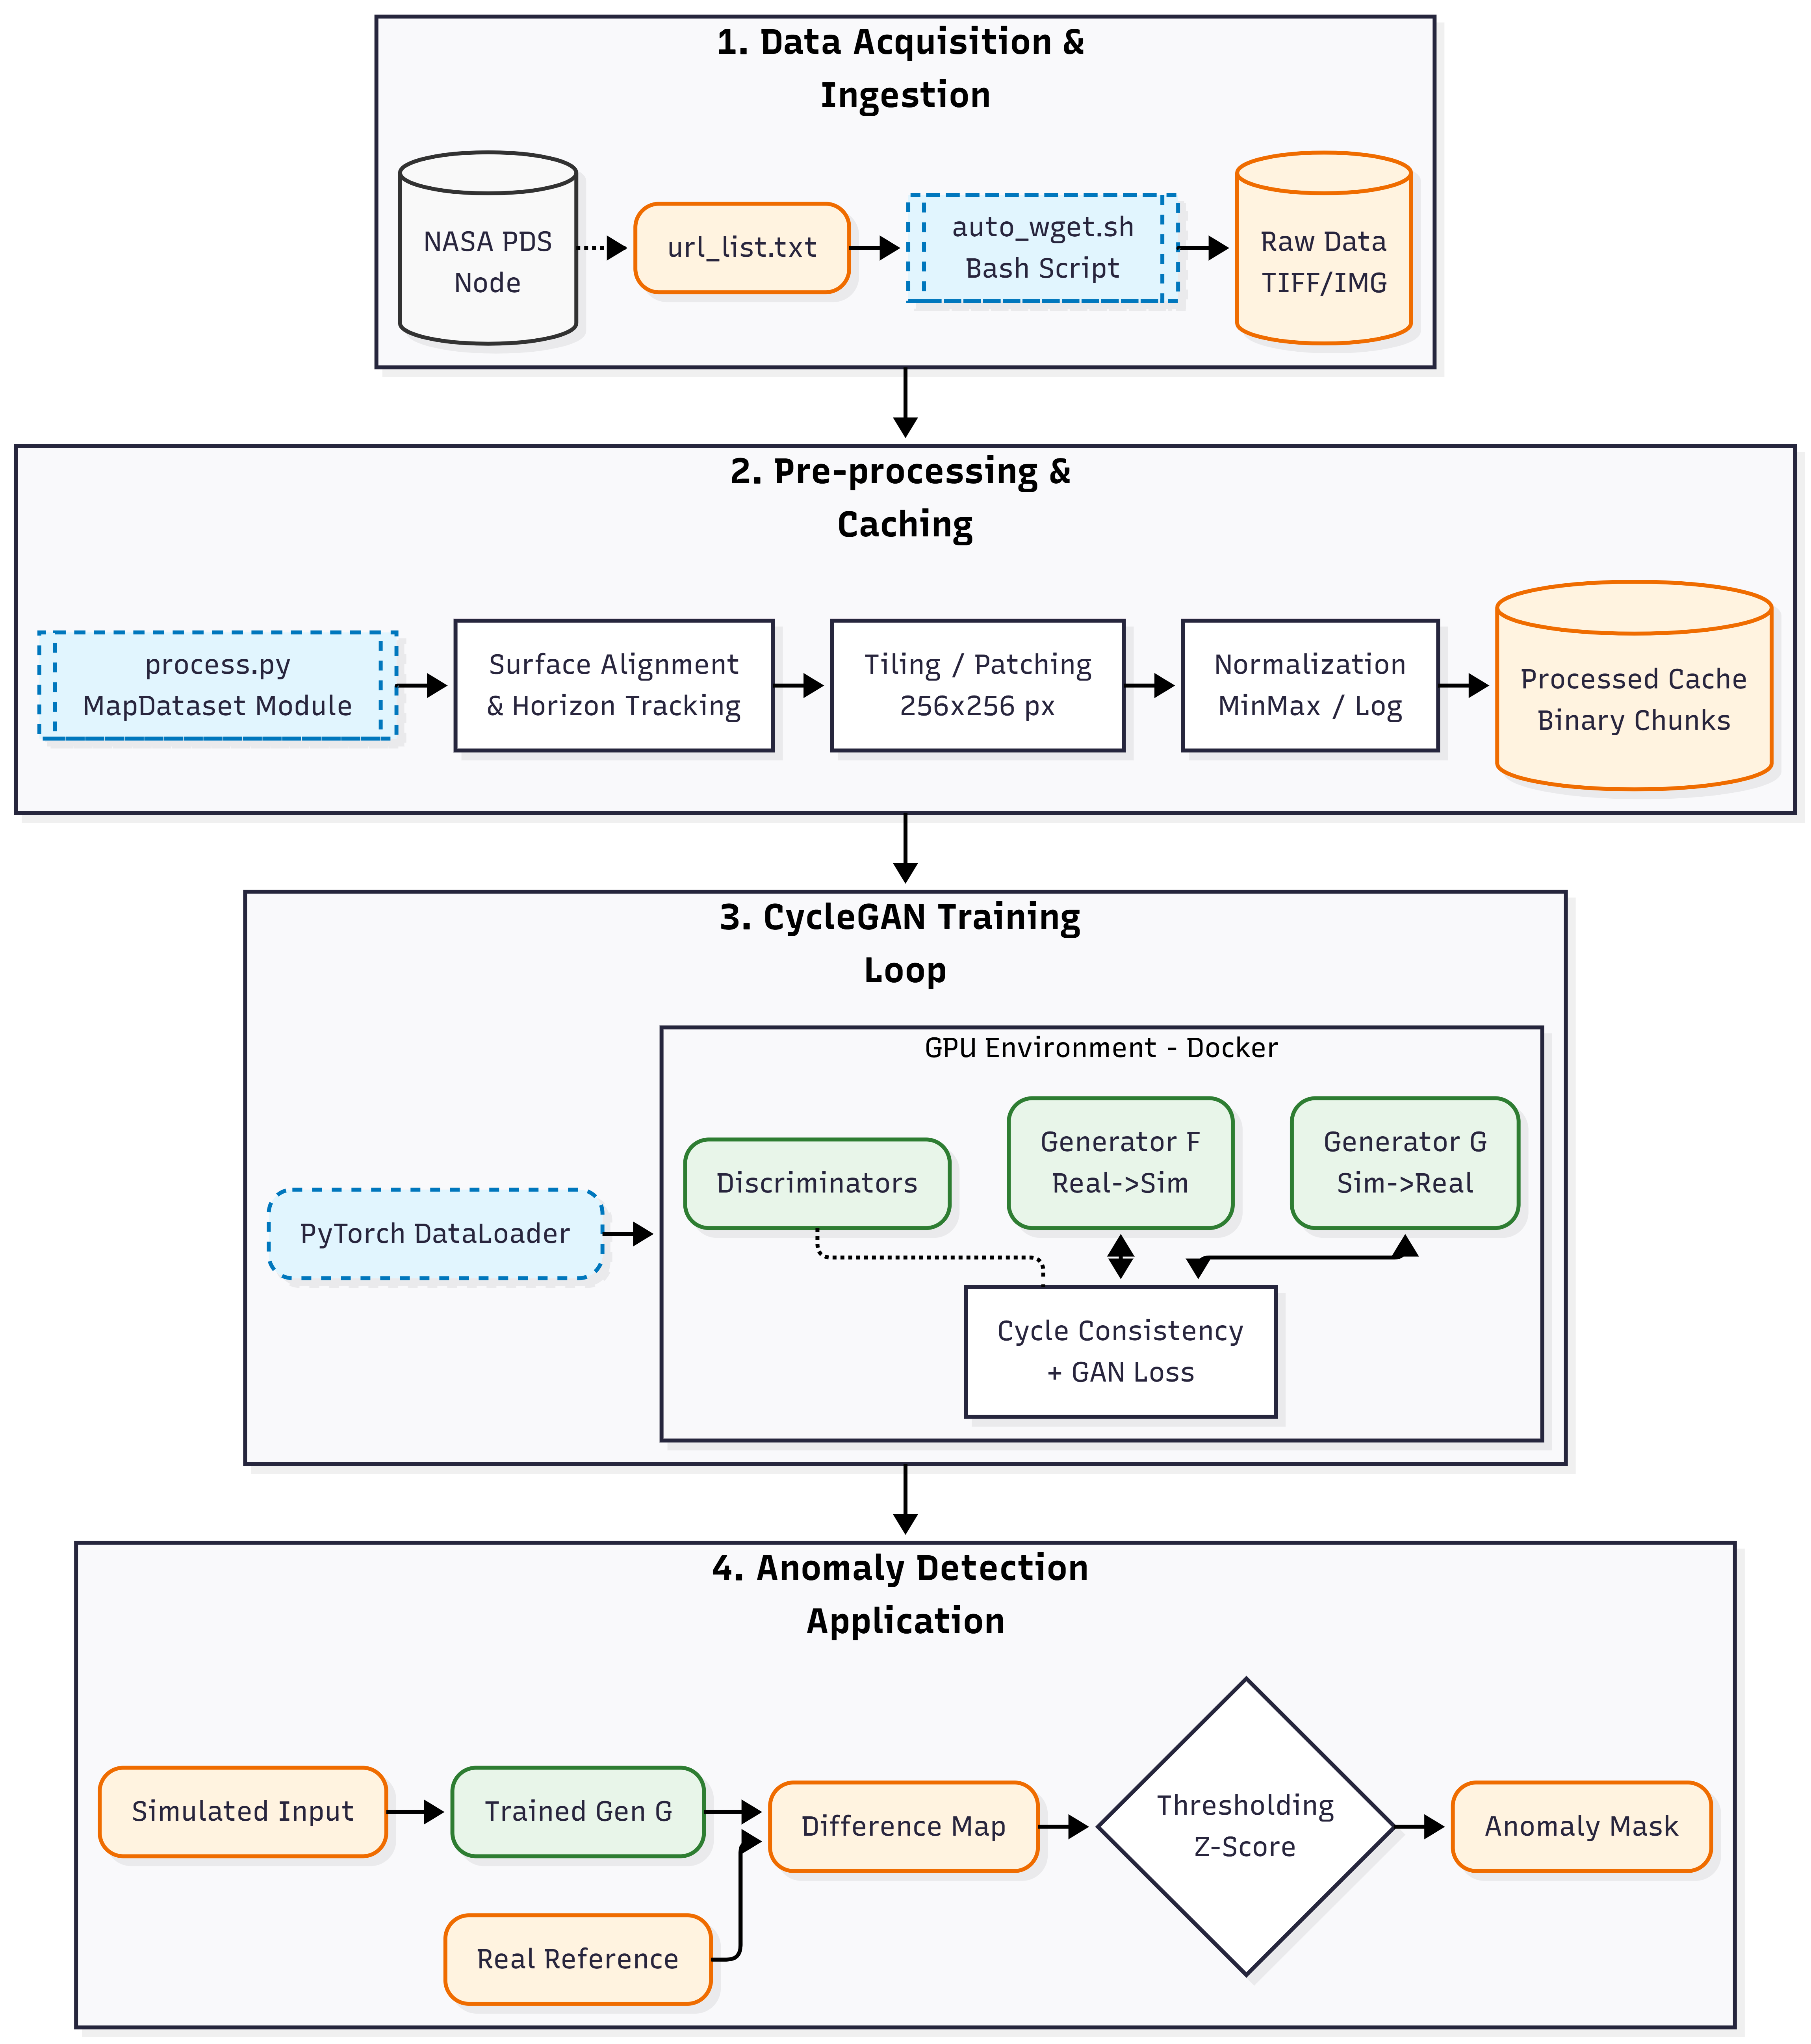
\includegraphics[width=\textwidth]{images/diagrams/high-level-system-architecture-V}
    \caption{High-level overview of the proposed system architecture. The pipeline encompasses automated data ingestion from NASA PDS (Block 1), pre-processing and efficient caching (Block 2), the CycleGAN training loop (Block 3), and the final anomaly detection application (Block 4).}
    \label{fig:system_architecture2}
\end{figure}

This modular architecture ensures that the computation-heavy pre-processing steps are decoupled from the training phase, allowing for rapid experimentation cycles once the cache is generated.

\subsection{Automated Data Acquisition}
To process the planetary-scale volume of SHARAD observations, manual data retrieval is structurally inadequate.
Consequently, a fully automated and parallelized acquisition pipeline was developed to interface directly with the NASA Planetary Data System (PDS) archives (see Block 1 of Figure~\ref{fig:system_architecture2}), which host the calibrated SHARAD radargrams and associated metadata for MRO~\cite{Zurek_2007,Seu_2007}.

The acquisition protocol is driven by a standardized manifest file (\texttt{url\_list.txt}) containing the Universal Resource Identifiers (URIs) of the target observations, ensuring complete experimental reproducibility.
To optimize the retrieval phase, the pipeline employs a concurrent fetching strategy (orchestrated via \texttt{auto\_wget.sh}) that maximizes network bandwidth utilization, drastically reducing the dataset initialization time. 

Given the massive scale of the data (often spanning hundreds of gigabytes) and the potential for network instability, the ingestion system is designed with strict fault-tolerance mechanisms.
It incorporates state-tracking to verify local data integrity prior to initiating transfers, thereby avoiding redundant downloads and allowing the ingestion process to be safely interrupted and resumed.
This robust data engineering foundation is essential to guarantee that the subsequent deep learning models are trained on a complete, uncorrupted representation of the target geological regions~\cite{yebasse2025advances}.

\subsection{Region of Interest (ROI) Selection: A Hybrid Strategy}
While the ingestion of raw data is fully automated, the specific selection of data segments for training and testing---the Regions of Interest (ROI)---followed a nuanced strategy that balances the massive data requirements of deep learning with the need for rigorous scientific evaluation.
This decision represents a deliberate trade-off between engineering automation, dataset size, and the \enquote{cleanliness} of the data distribution, as discussed in the context of SHARAD-based geological studies in~\cite{foss2017sharad3d,yebasse2025advances}.


\section{The Dataset: MRO SHARAD Radar Data}
\label{sec:dataset}
The primary dataset for this research is composed of RS data from the Shallow Radar (SHARAD) instrument~\cite{Seu_2007}, aboard NASA's Mars Reconnaissance Orbiter (MRO) \cite{Zurek_2007}.
SHARAD is a RS designed to probe the Martian subsurface, providing cross-sectional views (radargrams) of the planet's polar ice caps and layered deposits.
The data products are publicly available through the NASA Planetary Data System (PDS), the official archive for data from NASA's planetary missions~\cite{nasa_pds_geosciences}.

The SHARAD data products are provided in a format that includes \texttt{.xml} label files and associated binary data files.
The label files contain metadata describing the observation, while the binary files store the radargram.
In this 2D representation, one axis represents the along-track dimension (the sequence of radar pulses as the spacecraft moves) and the other axis represents the echo time delay, which is proportional to the depth of the reflecting feature.
The raw data values represent the power of the reflected signal. For visualization and analysis, these power values are typically converted to a logarithmic scale (decibels, dB) using the formula $P_{dB} = 10 \log_{10}(P_{linear})$.
This conversion compresses the vast dynamic range of the radar signals, making subtle subsurface features more discernible.

A key aspect of this project is the use of a paired dataset, which is essential for image-to-image translation tasks with models like Pix2Pix.
The dataset consists of two corresponding sets of images:
\begin{itemize}
    \item \textbf{Simulated Radar Data (Input)}: Synthetic radargrams generated via \textbf{incoherent geometric-optics ray-tracing} over Elysium Planitia DEMs~\cite{SimIncoherentRS2024}. The simulator traces rays from SHARAD's orbital trajectory to surface scatterers, computing power returns via the radar equation while neglecting subsurface propagation and phase interference. These simulations produce \enquote{clean} or idealized radargrams without speckle, matching SHARAD's orbital geometry. Each simulated radargram corresponds spatially to a real SHARAD observation acquired over identical topography.
    \item \textbf{Real SHARAD Data (Target)}: This consists of actual radargrams collected by the SHARAD instrument. These images contain complex noise patterns, surface clutter, subsurface reflectors, multiplicative speckle, and other artifacts resulting from the instrument's interaction with the Martian surface and subsurface.
\end{itemize}
Simulated inputs are perfectly spatially aligned with real targets via precise orbit-to-surface coordinate transforms.
Notice that these pairs are not calibrated in absolute power or SNR~\cite{Seu_2007}: simulated peak returns lack real instrument gain patterns, and subsurface-free simulations exhibit artificially high deep-SNR absent in observations.
We then apply dataset-wide logarithmic scaling/normalization (Section~\ref{sec:preprocessing_patching}) that equalizes dynamic range while preserving relative contrast essential for texture learning~\cite{Zhu_2017}.

This pairing allows the model to learn a direct mapping from the cleaner, simulated representation to noisy real-world data, thereby providing the foundation for the core methodological hypothesis: a generator trained to translate clutter-only simulations into realistic radargrams will systematically under-reconstruct genuine subsurface interfaces, which consequently emerge as high-confidence residuals suitable for unsupervised anomaly detection.


\section{Data Pre-processing and Patch Extraction Strategy}
\label{sec:preprocessing_patching}
The raw SHARAD radargrams are characteristically large, often extending to thousands of pixels in depth (e.g., $3600 \times N$, where 3600 represents the depth samples (fast-time, $\sim$9~km two-way travel) and $N \in [1000,5000]$ the variable along-track columns depending on orbit segment).
Training Convolutional Neural Networks (CNNs) directly on these full-scale images presents two significant challenges:
\begin{enumerate}
    \item \textbf{Computational Prohibitiveness:} The memory footprint required to process such large tensors via backpropagation exceeds the VRAM capacity of standard GPUs, drastically limiting batch sizes and increasing training time (a $3600 \times N$ FP32 tensor requires $\sim$3600$\times N \times$4~bytes, exceeding $\sim$24~GB VRAM and forcing batch size~1).
    \item \textbf{Sparse Information Density:} Radar signals suffer from attenuation as they penetrate the subsurface. Consequently, the useful geological information is highly concentrated in the upper portion of the radargram (near the surface reflection, within the first $\sim$300--500 pixels, corresponding to $\sim$10\% of the total depth range). The deeper sections are predominantly dominated by thermal noise. Training on the entire depth would force the network to process vast amounts of irrelevant noise, reducing learning efficiency.
\end{enumerate}


\begin{figure}[htbp]
    \centering
    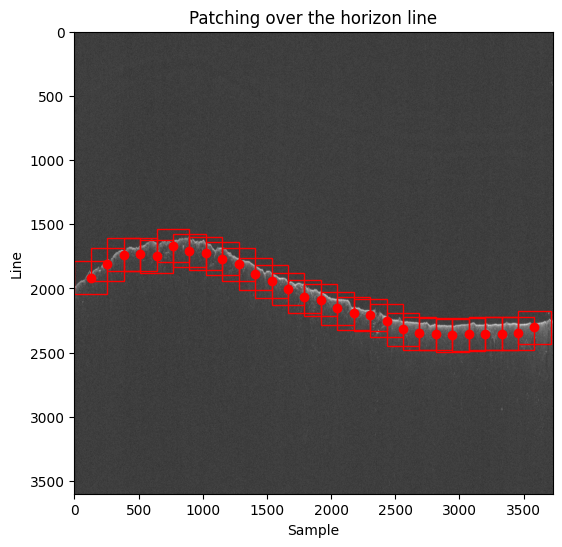
\includegraphics[width=\linewidth]{images/example_plots/ID_01970402/patching_example}
    \caption{Surface-aware patch extraction of sample with ID 01970402. Red markers indicate center of the box; colored boxes show extracted overlapping patches (28 total, 50\% overlap).}
    \label{fig:patch_extraction_column4160}
\end{figure}

To address these issues, a custom \textbf{Surface-Aware Patch Extraction} algorithm was implemented (executed via the \texttt{process.py} script, corresponding to the workflow in Block 2 of Figure~\ref{fig:system_architecture2}).
This strategy extracts square patches (fixed size $H \times W$, e.g., $128 \times 128$) focused specifically on the scientifically relevant subsurface regions.

The extraction procedure consists of four steps:
\begin{itemize}
    \item automated peak-finding identifies the surface reflection horizon across the azimuth dimension.
    \item a dynamic bounding box extracts a square patch (e.g., $128 \times 128$ pixels) below the top edge, capturing the relevant subsurface regions while rejecting non-informative atmospheric returns.
    \item verlapping patches are drawn with a 50\% stride ($W/2$), ensuring complete coverage and local redundancy.
    \item irregular binary structures are heuristically reconstructed or discarded, while extreme specular outliers are mitigated via robust Min-Max normalization (using the 1st and 99th percentiles) rather than explicit patch rejection.
\end{itemize}
Applied to Elysium Planitia observations, this pipeline yields $\sim$50k training patches while concentrating computational resources on signal-rich regions.

\begin{figure}[htbp]
    \centering
    \begin{subfigure}{\textwidth}
        \centering
        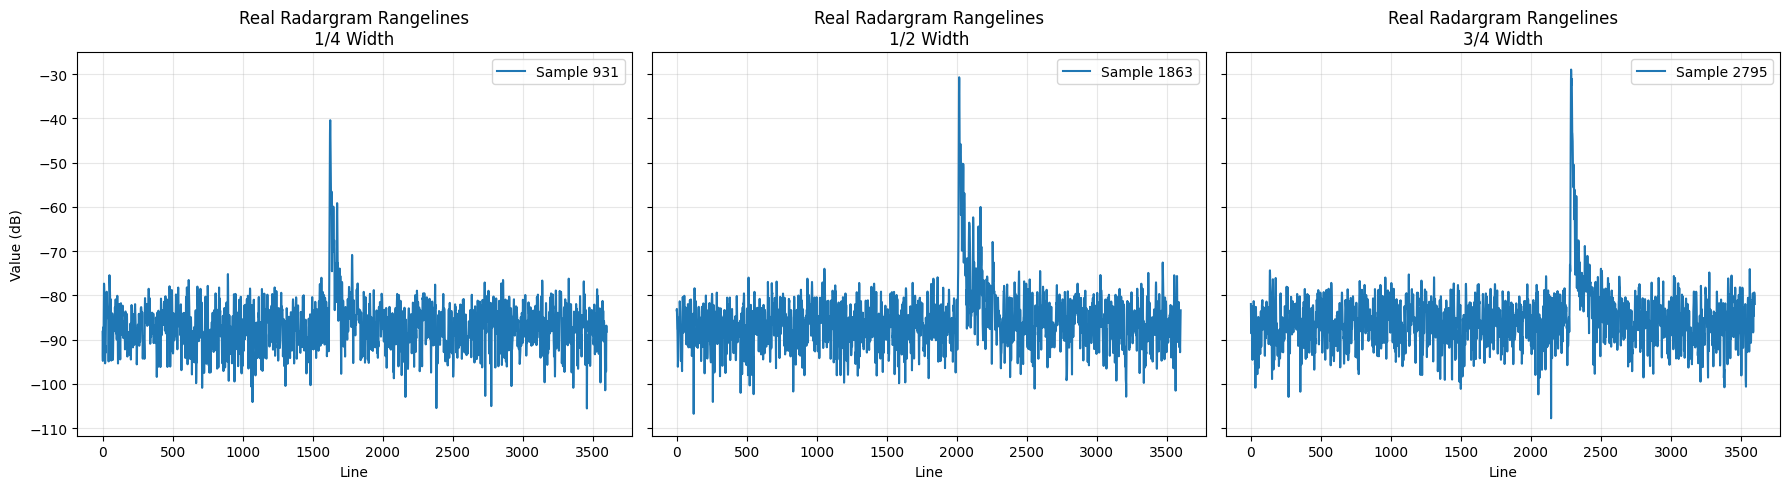
\includegraphics[width=\textwidth]{images/example_plots/ID_01970402/rangelines_real_db}
        \caption{Rangelines plotted in decibel (dB) scale. The profiles correspond to 0.25, 0.50, and 0.75 of the image width. A pronounced surface reflection is observed at approximately $-30$ to $-40$\,dB, whereas the majority of the signal is dominated by thermal noise around $-100$\,dB, illustrating sparse information density.}
        \label{fig:rangeline_sparse_density_db}
    \end{subfigure}
    
    \vspace{0.5em}
    
    \begin{subfigure}{\textwidth}
        \centering
        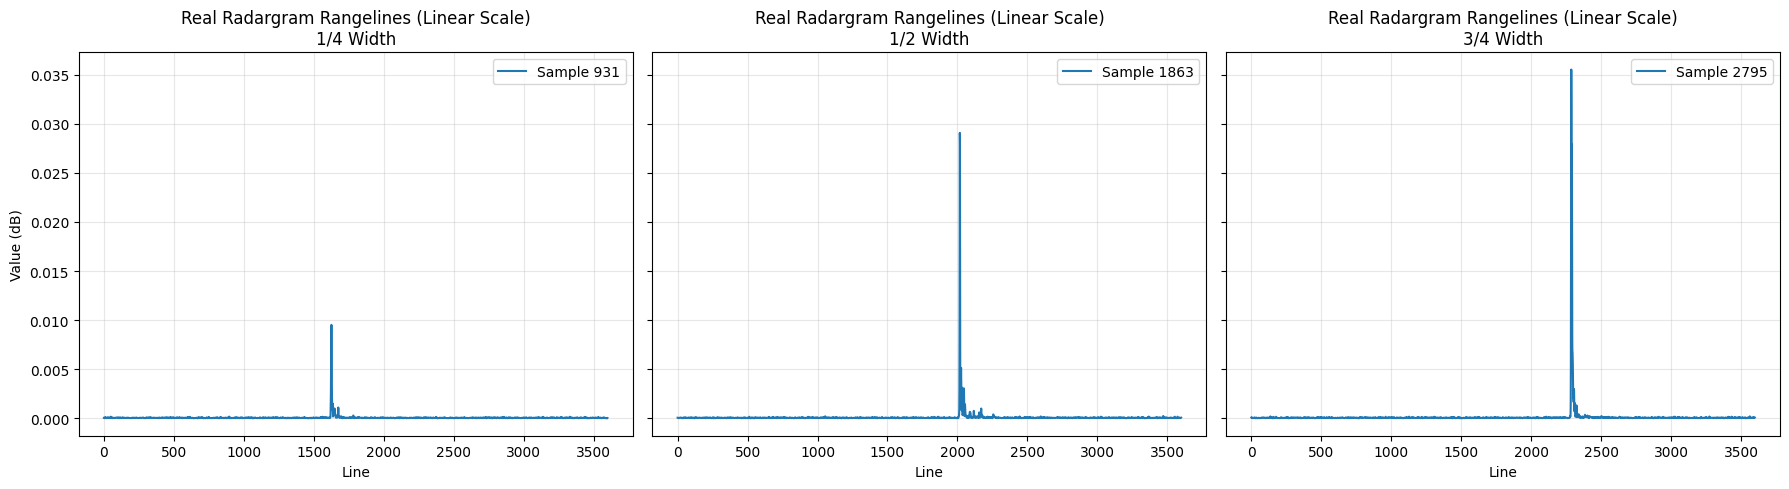
\includegraphics[width=\textwidth]{images/example_plots/ID_01970402/rangelines_real_linear}
        \caption{The same rangelines represented on a linear amplitude scale. The contrast between the surface reflection and the background noise becomes more pronounced, highlighting the large dynamic range of the signal.}
        \label{fig:rangeline_sparse_density_linear}
    \end{subfigure}
    
    \caption{Comparison of representative rangelines extracted at 0.25, 0.50, and 0.75 of the image width, shown in (a) logarithmic (dB) and (b) linear amplitude scales. The logarithmic representation emphasizes the noise floor and relative signal levels, while the linear representation accentuates the dominance of the surface reflection, demonstrating the sparse distribution of high-amplitude information within the scene.}
    \label{fig:rangeline_sparse_density}
\end{figure}

\subsection{Logarithmic Scaling and Dynamic Range Compression}
Radar signals are characterized by an extremely wide dynamic range, where the power of reflected echoes can span several orders of magnitude.
The specular reflection from the Martian surface often exhibits power levels millions of times greater than the faint dielectric contrasts of subsurface layers or the thermal noise floor.
If processed on a raw linear scale, these subtle subsurface features, which represent the primary targets of the present investigation, would be effectively invisible, quantized to the lowest values in a standard floating-point definition or lost entirely in the lower bits of an image format.

To address this, before patch extraction the first step in the pre-processing pipeline is the conversion of the linear power values, $P_{linear}$, into a logarithmic scale using the decibel (dB) unit.
This transformation is defined by the following equation:
$$ P_{dB} = 10 \log_{10}(P_{linear} + \epsilon) $$
where $\epsilon$ is a strictly positive infinitesimal constant (e.g., $10^{-13}$) to ensure numerical stability when $P_{linear} = 0$.

\subsection{Min-Max Normalization and Outlier Handling}
\label{subsec:minmax_normalization}
Deep learning models, particularly Generative Adversarial Networks (GANs), require input data to be normalized within a specific, bounded range to ensure stable gradient propagation.
The activation functions utilized in the generator (specifically the hyperbolic tangent, $\tanh$) and the discriminator typically operate most effectively when inputs are centered around zero with unit variance, or bounded within $[-1, 1]$.

In this framework, we adopt a Min-Max normalization strategy to rescale the decibel specifications to the $[-1, 1]$ interval. The transformation is given by:
\[ 
P_{norm} = 2 \frac{P_{dB} - v_{min}}{v_{max} - v_{min}} - 1 
\]
where $v_{min}$ and $v_{max}$ represent the global minimum and maximum power values observed across the entire training dataset.
It is crucial to note the statistical implications of this approach in the context of radar data.
Unlike natural images, where pixel values are naturally bounded (e.g., 0-255), radar power is theoretically unbounded.
In practice, coherent noise artifacts or specular reflections from orbital positioning maneuvers can produce "outliers" with anomalously high energy.
If $v_{max}$ is determined solely by the single brightest pixel in the entire dataset, a single artifact could stretch the normalization range excessively.
This would compress the vast majority of meaningful geological data into a tiny fraction of the $[-1, 1]$ range (e.g., $[-1, -0.9]$), effectively destroying the contrast required for the network to learn textures.
To mitigate this risk, our implementation calculates $v_{min}$ and $v_{max}$ using the 1st and 99th percentiles of the data distribution across the entire dataset.
This robust statistical approach ensures that the normalization range is determined by the geological signal rather than by transient instrument anomalies.

\begin{figure}[htbp]
    \centering
    \begin{subfigure}{\textwidth}
        \centering
        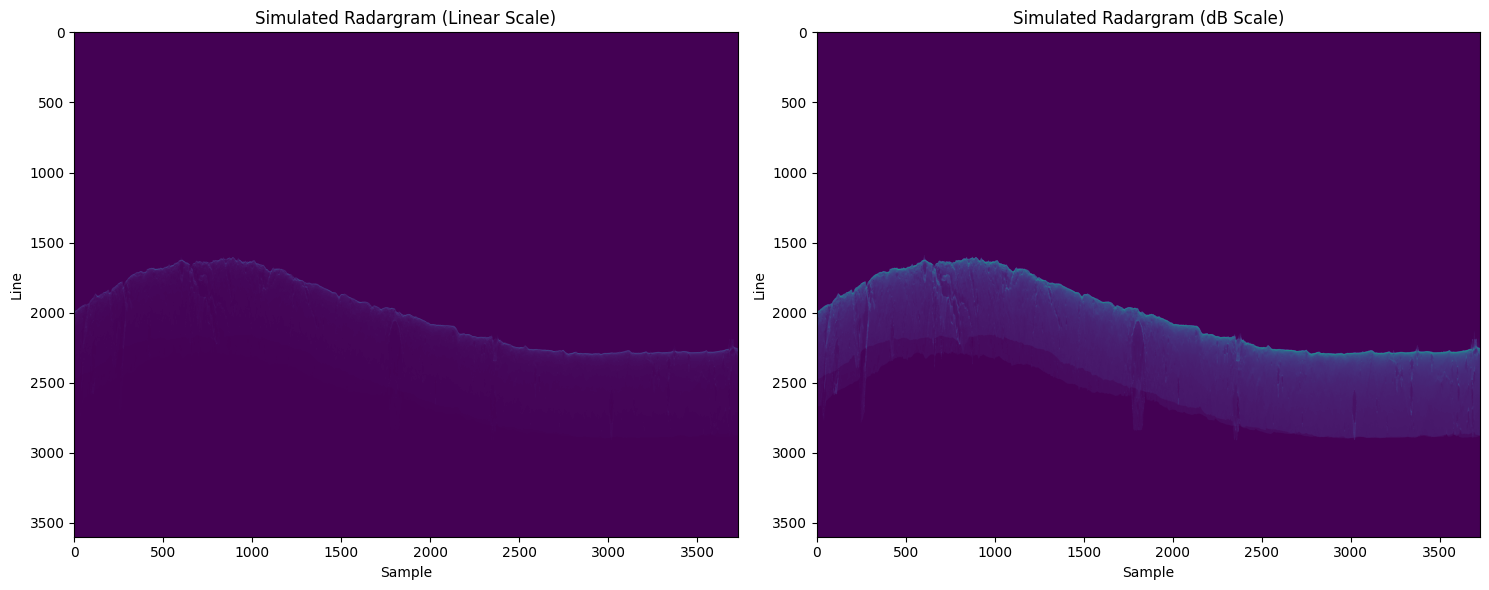
\includegraphics[width=\textwidth]{images/example_plots/ID_01970402/linear_vs_db_sim_RGB}
        \caption{Comparison using simulated SHARAD data. The left image shows the data in linear power scale; the right image in dB scale.}
        \label{fig:log_scaling_sim}
    \end{subfigure}
    
    \vspace{0.5em}
    
    \begin{subfigure}{\textwidth}
        \centering
        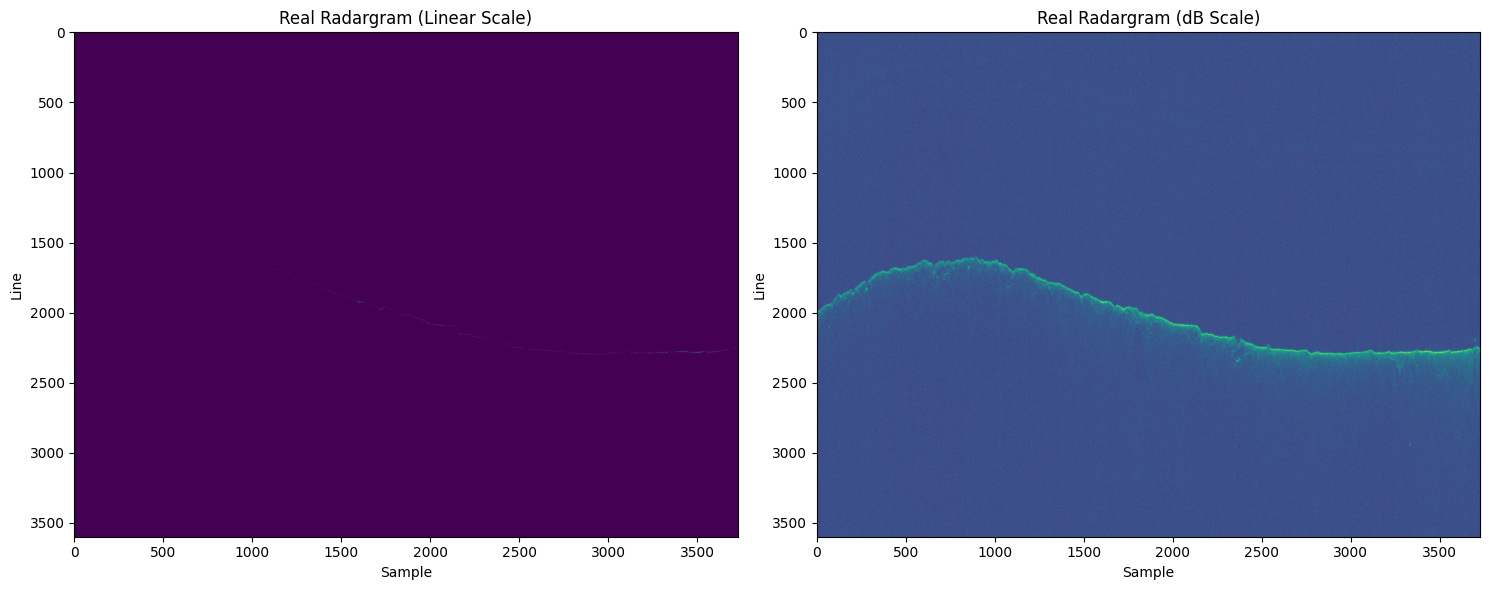
\includegraphics[width=\textwidth]{images/example_plots/ID_01970402/linear_vs_db_real_RGB}
        \caption{Comparison using real SHARAD data. The left image shows the data in linear power scale; the right image in dB scale.}
        \label{fig:log_scaling_real}
    \end{subfigure}
    
    \caption{Comparison of real and simulated SHARAD radargrams, each presented in (left) linear power scale and (right) logarithmic (dB) scale. (a) shows simulated data, (b) shows real data. For both, the linear plots are rendered using a dynamic range normalization (such as a median-based approach common in visualization libraries), causing the high-intensity surface reflection to be completely obscured by the statistical dominance of low-power subsurface and atmospheric returns. In the linear plot of the real data (b), the surface is invisible, while in the simulated data (a) it is only faintly visible. The dB transformation effectively compresses the dynamic range, providing numerical and perceptual accessibility to low-power geological features and a useful range for all information within the scene.}
    \label{fig:log_scaling_comparison}
\end{figure}

\subsection{Choice of the Data Normalization Strategy}
\label{subsec:ablation_normalization_study}
To justify the pre-processing decisions detailed in the previous subsections, we conducted an ablation study to compare three normalization approaches and their impact on the GAN's ability to generate realistic subsurface textures.
We recall that, unlike standard RGB images, radar data represents echo power with a potentially infinite dynamic range.

\subsubsection{Tested Approaches}
\begin{enumerate}
    \item \textbf{Method A: Linear Min-Max (Naive)}
    $$ x_{norm} = \frac{x - x_{min}}{x_{max} - x_{min}} $$
    Here, the raw power values are scaled linearly to [0, 1].
    
    \item \textbf{Method B: Z-Score Standardization}
    $$ x_{norm} = \frac{x - \mu}{\sigma} $$
    This centers the data around 0 with unit variance, common in many deep learning tasks.
    
    \item \textbf{Method C: Logarithmic Scaling + Min-Max (Proposed)}
    $$ x_{dB} = 10 \log_{10}(x + \epsilon) $$
    $$ x_{norm} = \frac{x_{dB} - \min(x_{dB})}{\max(x_{dB}) - \min(x_{dB})} $$
    The data is first converted to decibels (dB) to compress the dynamic range, and then scaled to $[-1, 1]$.
\end{enumerate}

\subsubsection{Results and Discussion}
The experiments revealed drastic differences in the quality of the learned distributions:

\begin{itemize}
    \item \textbf{Effect of Linear Scaling (Method A):} Radar data is dominated by the strong surface reflection, which can be orders of magnitude stronger than subsurface echoes. When using linear scaling, the surface peak sets the $x_{max}$ to a very high value, causing all faint subsurface features to be compressed into a tiny range near zero. Visually, the radargrams appeared almost black with a single white line (the surface). GANs trained on this data failed completely, learning only to generate a black background.
    \item \textbf{Effect of Z-Score (Method B):} While better than linear scaling, Z-score does not bound the data to a fixed range (e.g., $[-1, 1]$). Outliers (strong reflections) resulted in extreme values that pushed the \texttt{tanh} activation function into its saturation regions, leading to unstable training. This was primarily because the logarithmic transformation was not applied in this case, leading to ultimately worse performance than Method C.
    \item \textbf{Success of Logarithmic Scaling (Method C):} The logarithmic transformation naturally aligns with the physics of wave attenuation, compressing the orders of magnitude of power difference into a linear decibel scale. When combined with Min-Max scaling to $[-1, 1]$, it provided the optimal input for the network. The GAN successfully learned to distinguish and reproduce both the strong surface reflection and the delicate subsurface textures, as we will show in Chapter~\ref{cha:results}.
\end{itemize}

This study confirms that logarithmic pre-processing is not just an enhancement but a strict requirement for the convergence of GANs on radar sounding data.
We believe this is the driver of the success of Method C and it may also be applied to methods A and B.

\subsection{Surface Tracking Algorithm}
After normalizing the data, we perform a surface extraction process.
It is defined in the project's codebase (specifically \texttt{src/dataset/processing.py}), and uses an intelligent sliding window approach that adapts to the topography of the Martian surface.
For a given column $x$ in the radargram $R$, the algorithm identifies the surface horizon $y_{surf}$ as the index of the maximum signal intensity:
$$ y_{surf}(x) = \arg\max_j R(j, x) $$

A bounding box is then calculated to define the patch boundaries.
The vertical position of the box is not fixed but dynamically adjusted based on the local topography within the window width $W$.
The algorithm computes the minimum ($y_{min}$) and maximum ($y_{max}$) horizon depth within the interval $[x - W/2, x + W/2]$ to determine a \texttt{top\_edge}.
From this upper boundary, the bounding box extends downwards by a fixed patch height $H$.
This parameter $H$ is crucial as it defines the maximum depth of the geological context provided to the model.
The resulting extracted patch has fixed dimensions of $W \times H$, a design that ensures the surface interface is always contained within the upper portion of the patch, while maximizing the inclusion of the subsurface layers below it.

\begin{figure}[htbp]
    \centering
    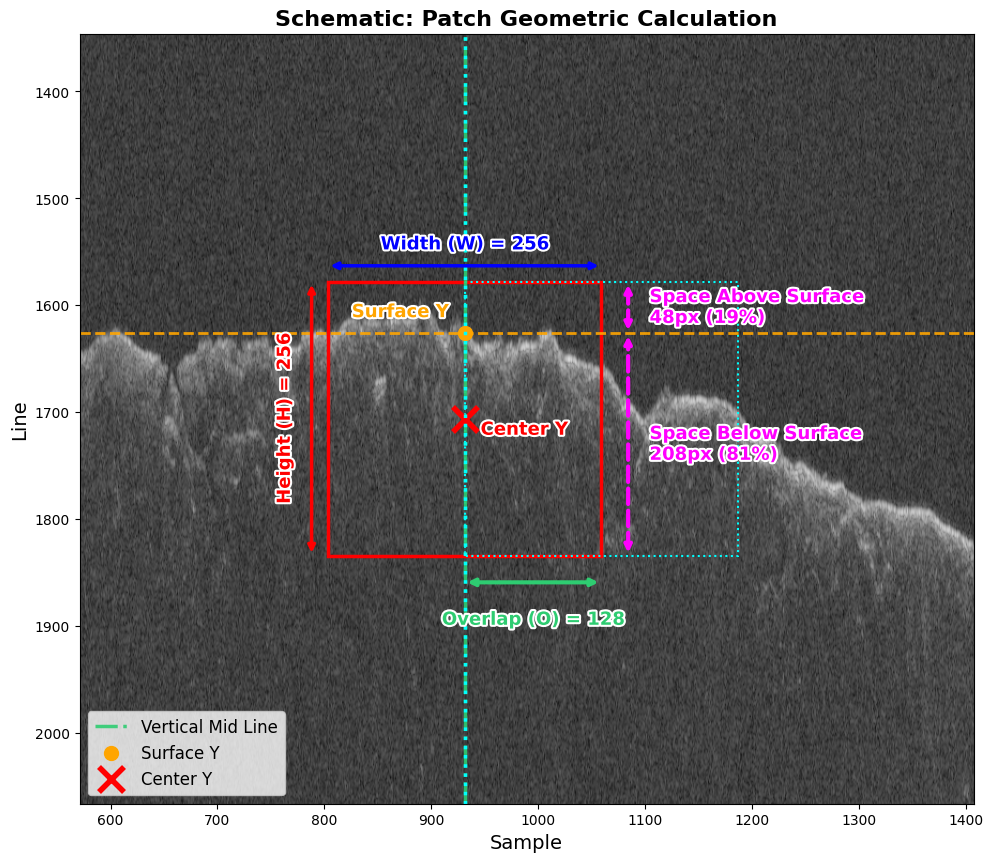
\includegraphics[width=0.8\textwidth]{images/example_plots/ID_01970402/patch_schematic}
    \caption{Illustration of the sliding window and patching mechanism on a Martian radargram. The red line represents the tracked surface $y_{surf}$. The highlighted bounding box demonstrates the extraction of a single patch of width $W$ and height $H$, starting from the dynamically adjusted \texttt{top\_edge}.}
    \label{fig:patching_logic}
\end{figure}

\subsection{Sliding Window and Overlap}
To prevent data loss at the boundaries of the patches---a common issue known as the \enquote{edge effect} where predictions degrade near the image borders---the patches are extracted with a significant overlap.
The stride $S$ of the sliding window is defined as:
$$ S = W - O $$
where $O$ is the overlap parameter (typically $W/2$).
This ensures that every geological feature appears in multiple patches, often centered in at least one, allowing the network to learn robust features invariant to their relative position in the input window.
Importantly, $O$ is not chosen too large to prevent samples from being too correlated with each other while still maintaining a reasonable number of independent samples for training.

\subsubsection{Handling Irregular Data Structures}
A significant practical challenge in the pre-processing pipeline was the intrinsic inconsistency of the raw PDS data products.
Although the SHARAD archive follows a well-defined standard, a non-negligible fraction of files exhibits irregularities in the binary layout, such as flattened arrays, non-standard padding, or truncated range lines.
If handled naively, these cases would either cause hard failures in the import stage or be silently discarded, effectively reducing the usable volume of the training dataset and biasing the statistics towards only the \enquote{cleanest} acquisitions.

To mitigate this issue, a custom heuristic procedure, implemented in the \texttt{handle\_irregular\_data} routine, was developed to reconstruct two-dimensional radargrams from such irregular binary arrays.
The algorithm operates in a multi-stage fashion.
First, it performs a consistency check against known SHARAD acquisition parameters by comparing the raw vector length with common radargram dimensions (e.g., $3600$ range samples per line) and their integer factors, noting that data in the PDS Object Description Exchange (ODE) is organized as a continuous stream of bytes rather than pre-formed 2D arrays.
When a direct reshape to $(N_{\text{range}}, N_{\text{azimuth}})$ is not possible, the routine estimates a plausible number of range samples by taking the median length over a local batch of products belonging to the same orbit or observation segment, under the assumption that their acquisition settings are identical.

In more pathological cases, the algorithm falls back to a brute-force factorization strategy: given a one-dimensional array of length $L$, it enumerates factor pairs $(n_r, n_a)$ such that $n_r \times n_a = L$ and favors configurations where $n_r$ is close to typical SHARAD values (e.g., $n_r \approx 3600$) while $n_a$ remains within a reasonable range for along-track extent.
Candidate reshapes are then validated by simple sanity checks on the resulting 2D image, such as verifying that the maximum power response lies near the expected surface region and that no entire rows or columns are saturated or identically zero.

If at least one configuration passes these heuristic tests, the corresponding reshaped radargram is accepted and forwarded to the subsequent logarithmic scaling and normalization stages described above; otherwise, the product is flagged as irrecoverable and excluded.
This robust handling of irregular data structures prevents the training pipeline from being halted by corrupted or non-standard PDS products and maximizes the amount of information that can be recovered from the archive, thereby increasing the statistical diversity and coverage of the final training set.


\section{Resource-Constrained Data Loading}
\label{sec:data_loading}
Handling a dataset of planetary scale introduces a classic Big Data engineering challenge: the total volume of processed data often exceeds the available Random Access Memory (RAM).
Attempting to load the entire dataset of high-resolution float32 tensors into memory would result in immediate system exhaustion (Out-Of-Memory errors).
To address this, a \textbf{Resource-Constrained Data Loading} architecture was implemented within the \texttt{MapDataset} class, leveraging lazy loading, memory-aware chunking, and incremental caching.

\subsection{Chunk-Based Memory Management}
Naive implementations often attempt to allocate a single contiguous memory block for the entire dataset, leading to memory fragmentation and OOM errors on consumer hardware.
The \texttt{MapDataset} instead structures the data as a list of independent tensor chunks (\texttt{self.data\_real}, \texttt{self.data\_sim}).
During the dataset construction phase, a \texttt{consolidate\_and\_free\_memory} routine monitors the process's Resident Set Size (RSS).
When memory usage exceeds a safety threshold (e.g., 4GB), the accumulated patches are consolidated into a tensor chunk and appended to the main list.
Crucially, the temporary build buffer is then explicitly cleared and the system's garbage collector is manually invoked.
This aggressive memory reclamation ensures that unreferenced data is immediately freed rather than waiting for background automated processes, preventing sudden memory spikes and allowing the system to process datasets arbitrarily larger than the available physical RAM.

\begin{figure}[htbp]
    \centering
    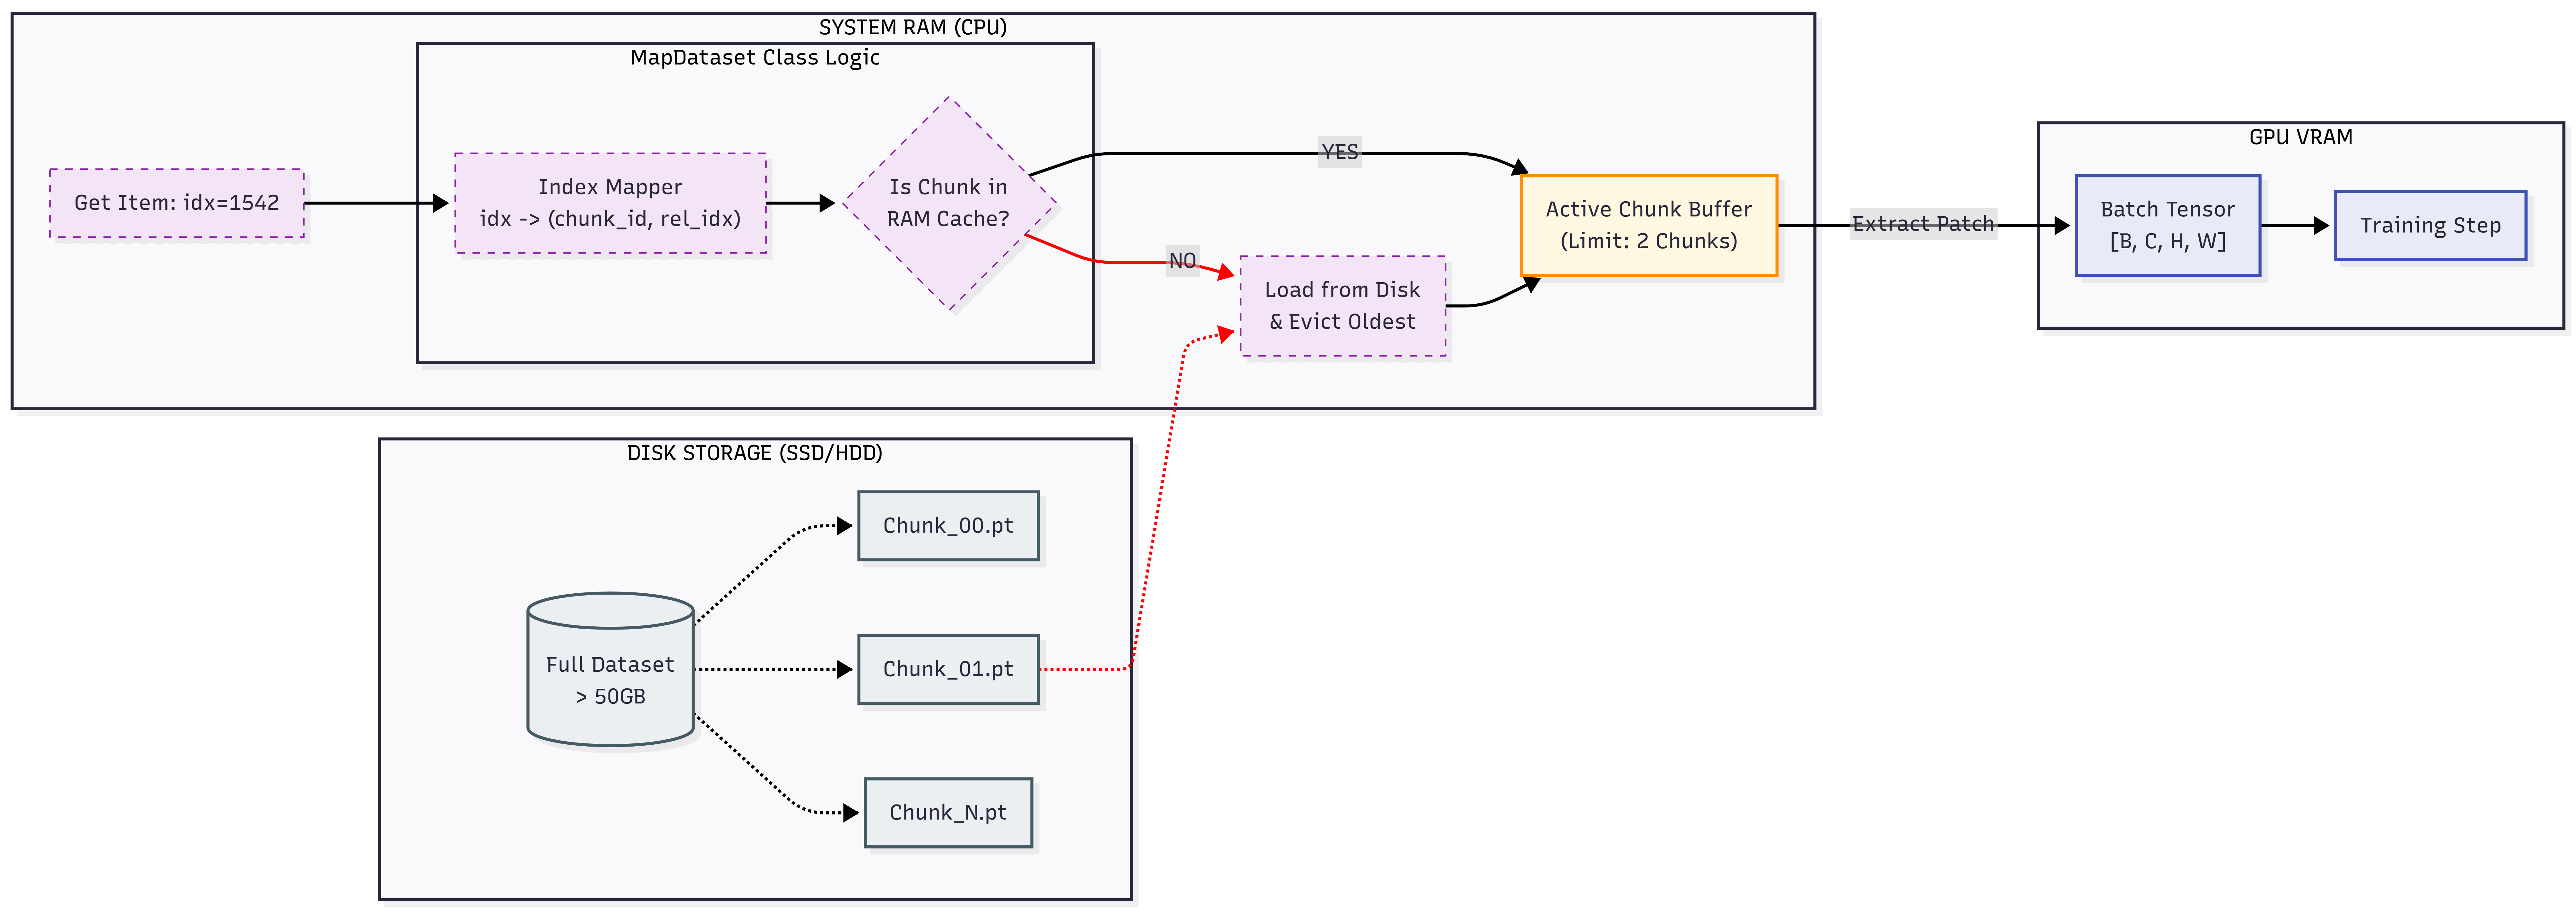
\includegraphics[width=\textwidth]{images/diagrams/memory-efficient-data-loading-strategy.png}
    \caption{Detail of the memory-efficient data loading strategy implemented in the MapDataset class. Large datasets are split into binary chunks on disk and dynamically loaded into a limited RAM buffer using a Least Recently Used (LRU) caching policy to enable training on consumer-grade hardware.}
    \label{fig:data_loading_strategy}
\end{figure}

\subsection{Two-Pass Incremental Build and Caching}
To eliminate the overhead of repeated pre-processing, the system implements a \textbf{Caching Mechanism}.
The \texttt{two\_pass\_incremental\_build} function orchestrates the dataset creation using a two-pass algorithm designed to minimize peak memory usage:

\begin{enumerate}
    \item \textbf{Pass 1 (Statistics):} The pipeline iterates through the entire raw dataset on disk to compute global normalization statistics (global Min/Max) without storing the images in memory. This ensures that the subsequent normalization is consistent across the entire dataset.
    \item \textbf{Pass 2 (Extraction):} The pipeline re-iterates to apply normalization and extract patches using the computed statistics. This phase utilizes a "streaming" approach, where patches are extracted, accumulated in chunks, and serialized to disk as independent \texttt{.pt} (PyTorch) binary archives.
\end{enumerate}

\subsection{Disk Caching and LRU Dynamic Loading Strategy}
For subsequent training runs, the system calculates a hash (MD5) of the current configuration (patch size, normalization type, etc.).
If the corresponding cache files matching this hash exist, the dataset is loaded directly from disk (\texttt{load\_from\_cache}), bypassing the raw data processing entirely.
This reduction in startup time—from hours to seconds—is critical for rapid experimental iteration.

Once the data is serialized into independent binary chunks on disk, their dynamic loading during the training phase is governed by a \textbf{Least Recently Used (LRU) caching policy}.
Instead of keeping all chunks in memory simultaneously, the \texttt{MapDataset} maintains a strictly bounded RAM buffer.
When a specific data patch is requested by the Dataloader, the system checks if its parent chunk is currently in the RAM cache.
If a cache miss occurs, the chunk is sequentially loaded from disk.
Should the RAM buffer be at maximum capacity, the LRU algorithm automatically deallocates the chunk that has not been accessed for the longest time, making room for the new one.
This strategy guarantees fast batch generation while keeping the memory footprint strictly within consumer-grade hardware limits.


\section{Neural Network Implementation}
\label{sec:modular_implementation}
The core of this research is a custom deep learning framework implemented in \textbf{PyTorch}.
We adopt a strict \textbf{Modular Object-Oriented Design} pattern.
The architecture is structured to ensure scalability, ease of debugging, and the seamless interchangeability of different generative components.

The implementation decouples the abstract definition of the models from the training logic and the data ingestion pipeline, as explicitly illustrated in Step 3 of the system architecture (Figure~\ref{fig:system_architecture2}).
The \texttt{src/models} package( refer to Appendix~\ref{app:codebase} for the comprehensive directory structure of the project) contains discrete modules for each architecture, where Generators and Discriminators are defined as independent \texttt{torch.nn.Module} classes.
This modularity allows for the dynamic instantiation of networks based on runtime configuration, facilitating comparative studies between different topological variants without altering the training loop.

\subsection{Overview of the Employed GANs}
As detailed in Section~\ref{sec:gan_theory}, the project implements two primary Generative Adversarial Network (GAN) architectures: Pix2Pix~\cite{Isola_2017} and CycleGAN~\cite{Zhu_2017}.
While both share the fundamental adversarial principle, a game between a Generator ($G$) trying to create realistic samples and a Discriminator ($D$) trying to distinguish them from real data (conceptually illustrated in Figure~\ref{fig:gen_disc_scheme}), they differ fundamentally in their structural design, generator topologies, and loss formulations.

\subsection{Pix2Pix: Paired Translation}
The Pix2Pix framework \cite{Isola_2017} serves as the baseline conditional model, designed for tasks where perfect pixel-to-pixel alignment exists between the source and target domains.

\begin{figure}[htbp]
    \centering
    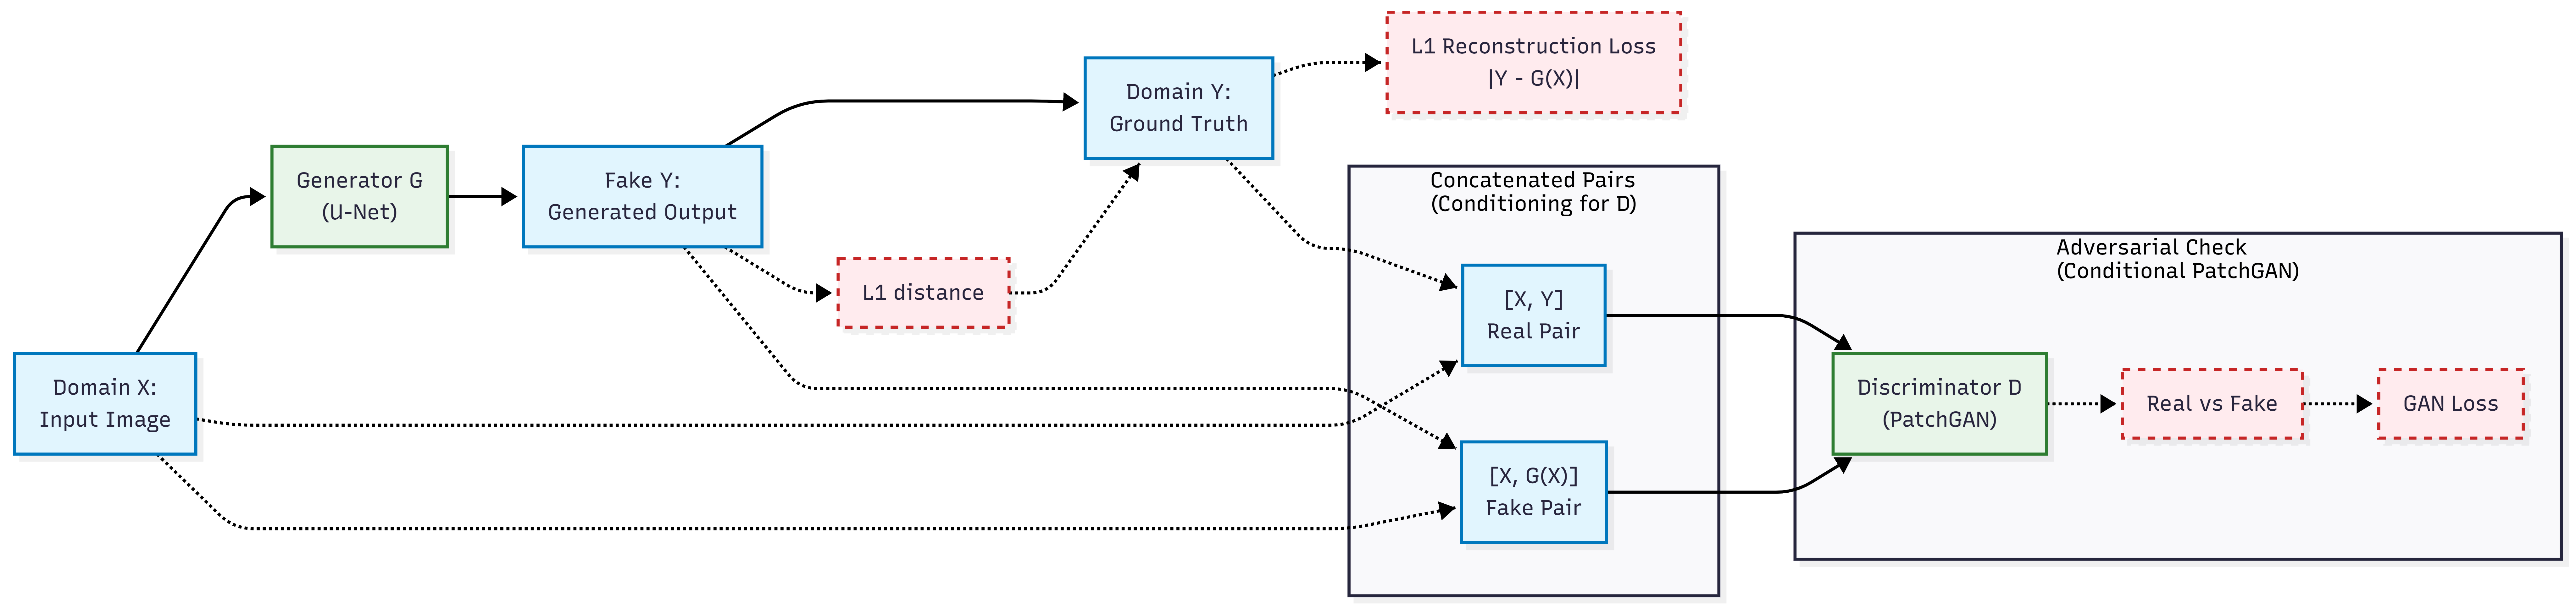
\includegraphics[width=\textwidth]{images/diagrams/pix2pix}
    \caption{Architecture of the Pix2Pix conditional GAN employed in the project. The generator translates simulated input maps into realistic radargrams efficiently using paired data supervision.}
    \label{fig:pix2pix_architecture}
\end{figure}

% \paragraph{Generator Architecture (U-Net with Skip Connections):}
\subsubsection{Generator Architecture: U-Net with Skip Connections}
\label{subsubsec:unet_generator}
The standard generator for the Pix2Pix model employs a modified \textbf{U-Net} architecture \cite{Ronneberger_2015}, a fully convolutional encoder-decoder network.
The complete topology of this network, including the downsampling bottleneck and the symmetric expansion path, was previously illustrated and detailed in Chapter~\ref{cha:preliminaries} (see Figure~\ref{fig:unet_architecture}).
The choice of U-Net is driven by the need to preserve low-level structural details (e.g., the precise depth of a subsurface interface) which are often lost in standard bottleneck architectures.

The \textbf{Encoder} is composed of 7 sequential blocks.
Each block typically consists of a Convolutional layer with a $4 \times 4$ kernel and stride 2 (performing spatial downsampling), followed by Instance Normalization and a LeakyReLU activation (slope 0.2).
This progressively compresses the $128 \times 128$ input into a latent feature representation of size $1 \times 1 \times 512$. 

The \textbf{Decoder} mirrors this structure using Transposed Convolutions (Deconvolutions) to upsample the feature maps back to the original resolution.
The critical innovation of the U-Net is the introduction of \textbf{Skip Connections}.
These connections concatenate the feature map from the $i$-th layer of the encoder directly to the $(n-i)$-th layer of the decoder.
Mathematically, if $E_i$ is the output of the encoder layer $i$, the input to the decoder layer $j$ becomes $[D_{j-1}, E_{n-j}]$.
This allows the unmodified high-frequency spatial information to flow directly to the output, bypassing the bottleneck.
For radar data, this is indispensable, ensuring that thin, sharp features like stratigraphic horizons are not blurred by the compression process.

\paragraph{Pix2Pix Loss Formulation:}
The objective of the Pix2Pix architecture combines a conditional adversarial loss with a traditional pixel-wise reconstruction loss, leveraging the availability of perfectly paired data.

\textbf{1. Conditional Adversarial Loss:}
Unlike a standard GAN that generates data from random noise, the conditional discriminator $D$ evaluates pairs of images: the input simulation $x_{sim}$ and either the real ground-truth radargram $x_{real}$ or the generated radargram $x_{gen} = G(x_{sim})$.
The generator $G$ tries to minimize this objective, while $D$ tries to maximize it:
$$ \mathcal{L}_{cGAN}(G, D) = \mathbb{E}_{x_{sim}, x_{real}}[\log D(x_{sim}, x_{real})] + \mathbb{E}_{x_{sim}}[\log(1 - D(x_{sim}, G(x_{sim})))] $$

\textbf{2. L1 Distance Loss:}
The adversarial loss alone is sufficient to generate sharp images, but it does not guarantee that the structural content matches the input.
To ensure the generated image captures the exact low-frequency structures (e.g., the correct depth of stratigraphic lines), an L1 regularization term is added.
It forces the generated image to be as close as possible to the ground truth at the pixel level:
$$ \mathcal{L}_{L1}(G) = \mathbb{E}_{x_{sim}, x_{real}}[\|x_{real} - G(x_{sim})\|_1] $$

The final objective for the Pix2Pix model is:
$$ \mathcal{L}_{Pix2Pix}(G, D) = \arg\min_G \max_D \mathcal{L}_{cGAN}(G, D) + \lambda \mathcal{L}_{L1}(G) $$
where $\lambda$ is a hyperparameter that controls the relative importance of the L1 term (typically $\lambda=100$, ensuring that structural fidelity dominates over pure adversarial realism).

\subsection{CycleGAN: Unpaired Translation}
The CycleGAN architecture \cite{Zhu_2017} represents a more sophisticated approach, removing the requirement for paired training data.
This is achieved by introducing two mapping functions: $G: X \rightarrow Y$ (Sim to Real) and $F: Y \rightarrow X$ (Real to Sim), and two discriminators $D_Y$ and $D_X$.

\begin{figure}[htbp]
    \centering
    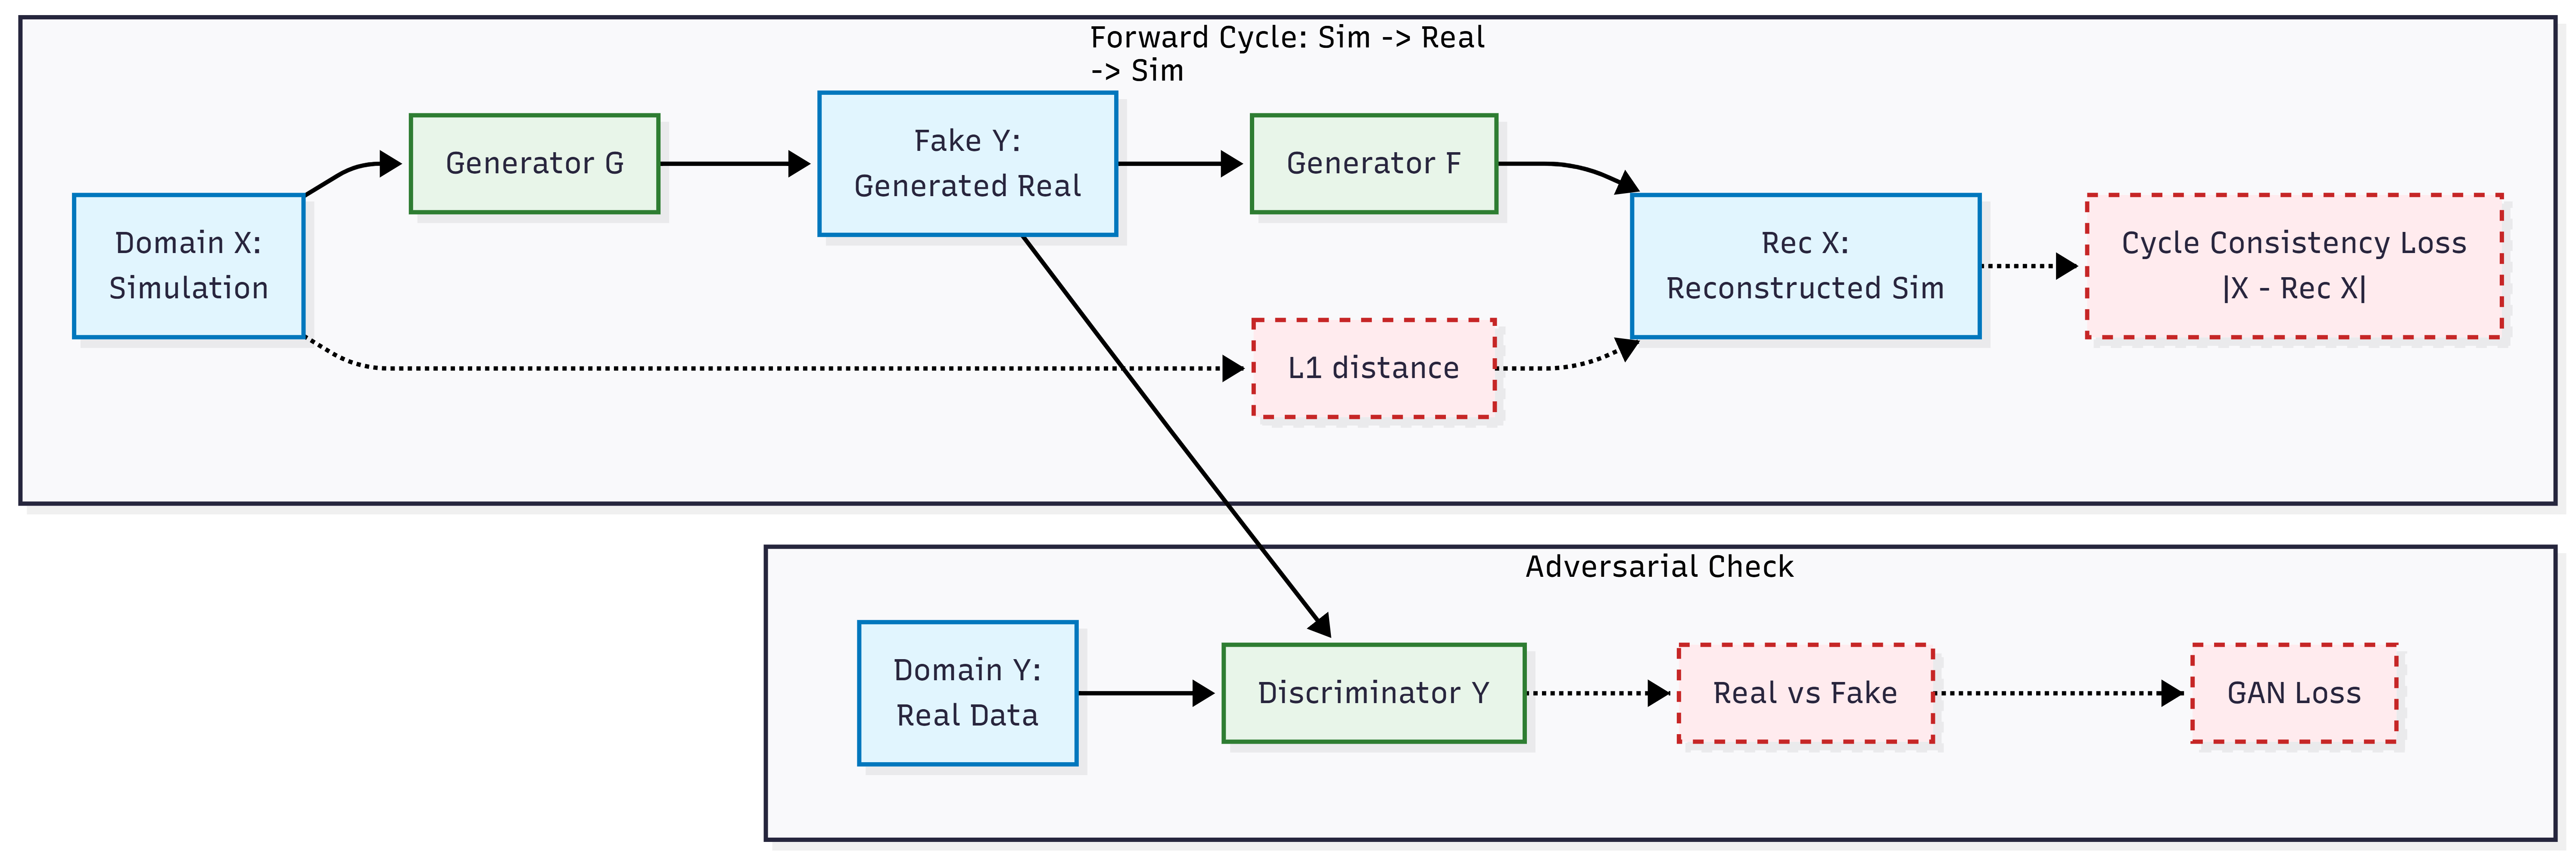
\includegraphics[width=\textwidth]{images/diagrams/cyclegan}
    \caption{Schematic of the CycleGAN architecture. The framework utilizes two generators and two discriminators to learn the mapping between simulated and real domains without paired examples, enforcing cycle consistency to preserve structural integrity.}
    \label{fig:cyclegan_architecture}
\end{figure}

\paragraph{Generator Architecture Variations:}
While CycleGAN can theoretically employ the same U-Net generator described in Section~\ref{subsubsec:unet_generator}, standard unpaired translation often favors a \textbf{ResNet-based} generator.
Unlike U-Net, which relies on direct skip connections between the encoder and decoder, ResNet transforms the features sequentially through residual blocks.
This prevents the network from aggressively copying the input via skip connections, avoiding artifacts in unpaired settings where the source and target are not perfectly aligned.
Thanks to the modularity of our framework, both U-Net and ResNet topologies are supported and can be dynamically instantiated.

\paragraph{CycleGAN Loss Formulation:}
The training objective of the CycleGAN architecture is a weighted sum of three distinct loss components, each serving a specific theoretical purpose to overcome the lack of paired supervision.

\textbf{1. Adversarial Loss:}
This standard GAN loss forces the generated images to be indistinguishable from real images.
For the mapping $G: \mathcal{X}_{sim} \rightarrow \mathcal{X}_{real}$, the objective is:
$$
\mathcal{L}_{GAN}(G, 
D_{real}, 
\mathcal{X}_{sim}, 
\mathcal{X}_{real})
=
\mathbb{E}_{x_{real}}
[\log D_{real}(x_{real})]
+
\mathbb{E}_{x_{sim}}
[\log(1 - D_{real}(G(x_{sim})))]
$$
Here, $G$ tries to minimize this objective (generate realistic samples), while $D_Y$ tries to maximize it (correctly classify real vs. fake).
A similar loss applies to the reverse mapping $F$.

\textbf{2. Cycle Consistency Loss:}
This is the core innovation of CycleGAN.
It enforces the constraint that translating a sample to the other domain and back should yield the original sample—effectively enforcing \textbf{Transitivity}.
If we translate a simulation $x_{sim}$ to a pseudo-real radargram $G(x_{sim})$, and then translate that back to a simulation using the reverse generator $F(G(x_{sim}))$, we should recover $x_{sim}$.
$$
\mathcal{L}_{cyc}(G, F)
=
\mathbb{E}_{x_{sim}}
\left[\|F(G(x_{sim})) - x_{sim}\|_1\right]
+
\mathbb{E}_{x_{real}}
\left[\|G(F(x_{real})) - x_{real}\|_1\right]
$$
This loss uses the L1 norm ($\|\cdot\|_1$) to penalize pixel-level differences.
Geologically, this is what preserves the stratigraphy: the model cannot simply generate a random realistic radar image; it must generate one that structurally corresponds to the input so that it can be translated back.

\textbf{3. Identity Loss:}
Often overlooked, the identity loss is critical for color and intensity preservation.
It states that if the generator $G$ (which converts Sim to Real) is fed an image that is \textit{already} from the Real domain ($x_{real}$), it should leave it unchanged:
$$
\mathcal{L}_{identity}(G, F)
=
\mathbb{E}_{x_{real}}
\left[\|G(x_{real}) - x_{real}\|_1\right]
+
\mathbb{E}_{x_{sim}}
\left[\|F(x_{sim}) - x_{sim}\|_1\right]
$$
In the context of radar, this prevents the generator from arbitrarily inverting the color palette or drifting the signal intensity.
It stabilizes the training by enforcing that the mapping is continuous near the target domain manifold.

The final full objective function is a weighted combination:
$$ \mathcal{L}(G, F, D_X, D_Y) = \mathcal{L}_{GAN}(G, D_Y, X, Y) + \mathcal{L}_{GAN}(F, D_X, Y, X) + \lambda \mathcal{L}_{cyc}(G, F) + 0.5 \lambda \mathcal{L}_{identity}(G, F) $$
where $\lambda$ controls the relative importance of cycle consistency (typically $\lambda=10$).

\subsection{Configuration-Driven Design}
To ensure rigorous experimental control and avoid "magic numbers" hardcoded in the source, the framework adopts a \textbf{Configuration-Driven Design}.
The entire experimental state is defined by declarative YAML configuration files (e.g., \texttt{config.yaml}).

This system allows for the strict separation of code (logic) and experiment (parameters).
Hyperparameters such as learning rates ($2 \times 10^{-4}$), architecture-specific loss weights ($\lambda_{cycle}=10.0$, $\lambda_{L1}=100.0$), batch sizes, and optimization strategies (Adam $\beta_1=0.5$) are injected at runtime.
This design explicitly supports the \enquote{Clean Code} principle, ensuring that running a new experiment (e.g., changing the cycle loss weight) requires no modification to the Python codebase, thereby eliminating the risk of introducing bugs during parameter tuning.
A summary of the baseline hyperparameter configurations used for both Pix2Pix and CycleGAN is presented in Table~\ref{tab:hyperparams}.

\begin{table}[htbp]
\centering
\caption{Summary of the Hyperparameter Configurations for Pix2Pix and CycleGAN Training}
\label{tab:hyperparams}
\begin{tabular}{lccc}
\hline
\textbf{Hyperparameter} & \textbf{Pix2Pix} & \textbf{CycleGAN} & \textbf{Description} \\ \hline
Input Resolution & $128 \times 128$ & $128 \times 128$ & Spatial dimensions of patches \\
Batch Size & 1 & 1 & Constraints due to Memory \\
Generator Learning Rate & $2 \times 10^{-5}$ & $2 \times 10^{-4}$ & Fixed \\
Discriminator Learning Rate & $1 \times 10^{-5}$ & $1 \times 10^{-4}$ & Fixed \\
Optimizer & Adam & Adam & Adaptive Moment Estimation \\
$\beta_1, \beta_2$ & $0.5, 0.999$ & $0.5, 0.999$ & Momentum terms \\
$\lambda_{L1}$ & $100.0$ & -- & Weight for L1 reconstruction loss \\
$\lambda_{cycle}$ & -- & $10.0$ & Weight for consistency loss \\
$\lambda_{identity}$ & -- & $5.0$ & Weight for identity loss \\
Epochs & 40 & 60 &Total training duration \\ \hline
\end{tabular}
\end{table}

\subsection{Micro-Architecture Definition}
To ensure stable training dynamics and high-fidelity texture synthesis, the abstract architectures described above were instantiated with a specific micro-architecture that departs in several aspects from standard CNN designs used for natural images.
In particular, the CycleGAN generators were implemented as 9-block ResNet networks with reflection padding and instance normalization, while the discriminators adopt a fully convolutional PatchGAN configuration with a finite receptive field over local patches.

\begin{figure}[htbp]
    \centering
    \begin{tikzpicture}[
        node distance=1.5cm and 1.5cm,
        box/.style={rectangle, draw, minimum width=2.8cm, minimum height=1.2cm, align=center, thick, rounded corners=2pt},
        arrow/.style={-{Stealth}, thick}
    ]
    
    % ---- RIGA SUPERIORE (Generazione) ----
    \node (sim) [align=center] {Simulated \\ Data ($x_{sim}$)};
    \node (gen) [box, right=of sim, fill=blue!10] {\textbf{Generator} ($G$) \\ \footnotesize{U-Net / ResNet}};
    \node (fake) [align=center, right=of gen] {Fake Radargram \\ ($x_{gen} = G(x)$)};
    
    % ---- RIGA INFERIORE (Discriminazione) ----
    % Posiziono il discriminatore esattamente sotto il fake radargram
    \node (disc) [box, below=1.2cm of fake, fill=red!10] {\textbf{Discriminator} ($D$) \\ \footnotesize{PatchGAN}};
    % I dati reali entrano da sinistra verso il discriminatore
    \node (real) [align=center, left=of disc] {Real \\ Radargram ($x_{real}$)};
    % L'output esce a destra
    \node (out) [align=center, right=of disc] {Real/Fake \\ Prediction};

    % ---- COLLEGAMENTI (Frecce) ----
    \draw [arrow] (sim) -- (gen);
    \draw [arrow] (gen) -- (fake);
    
    % Freccia che scende dal Fake al Discriminatore
    \draw [arrow] (fake) -- (disc);
    % Freccia dai dati reali al Discriminatore
    \draw [arrow] (real) -- (disc);
    
    \draw [arrow] (disc) -- (out);
    
    % ---- BOX TRATTEGGIATO OPZIONALE ----
    % Raggruppa la fase di discriminazione (Real, Fake, Disc, Out) per evidenziarla
    \draw[dashed, gray, thick] ([xshift=-0.5cm, yshift=0.3cm]real.west |- fake.north) rectangle ([xshift=0.3cm, yshift=-0.3cm]out.south east);
    
    \end{tikzpicture}
    \caption{Abstract schematic of the adversarial training framework. The Generator synthesizes realistic representations from simulated inputs, while the Discriminator evaluates both generated samples and real observations, outputting a probability score. The competing objectives of these two networks drive the optimization process.}
    \label{fig:gen_disc_scheme}
\end{figure}

\paragraph{Generator: 9-block ResNet with reflection padding}
The generator network $G$ follows a Johnson-style residual architecture and can be decomposed into three stages: downsampling, residual transformation, and upsampling.
The input is a single-channel radar patch $x \in \mathbb{R}^{1 \times 128 \times 128}$, already normalized to the range $[-1, 1]$ by the pre-processing pipeline described in Section \ref{sec:preprocessing_patching}.

\textbf{Downsampling.} The first stage consists of an initial $7 \times 7$ convolution with stride $1$ and reflection padding, followed by two strided convolutions ($3 \times 3$, stride $2$) that progressively reduce the spatial resolution while increasing the number of feature maps.
Concretely, the feature dimensionality evolves from $1 \times 128 \times 128$ to $64 \times 128 \times 128$, then to $128 \times 64 \times 64$, and finally to $256 \times 32 \times 32$.
Each block is followed by Instance Normalization (IN) and a ReLU activation, which together help to stabilize training across the highly heterogeneous dynamic range of radar echoes.

\textbf{Residual bottleneck.} The core transformation is implemented by a stack of 9 sequential residual blocks.
Each residual block $R_i$ applies the mapping
\[
y = F(x) + x,
\]
where $F(\cdot)$ is realized by two $3 \times 3$ convolutional layers with reflection padding, each followed by Instance Normalization and ReLU (except for the last activation, which is omitted to preserve the residual nature of the connection).
The use of reflection padding is critical in the radargram setting: zero padding would introduce artificial discontinuities at the patch borders (sharp transitions from valid signal to constant zeros), which the PatchGAN discriminator rapidly learns to classify as \enquote{fake}.
This mechanism typically manifests as grid-like artifacts at patch boundaries when tiling full radargrams.
Reflection padding, by mirroring the signal at the borders, preserves the continuity of stratigraphic horizons across patch edges and reduces such tiling artifacts.

\textbf{Upsampling.} The final stage restores the original spatial resolution through two transposed convolution layers with kernel size $3$ and stride $2$, which upsample the feature maps from $256 \times 32 \times 32$ back to $64 \times 128 \times 128$.
These are followed by a final $7 \times 7$ convolution with reflection padding and a $\tanh$ activation function, mapping the output back to the normalized range $[-1, 1]$.
This design ensures consistency with the Min-Max normalization adopted in Section \ref{subsec:minmax_normalization} and avoids mismatch between network outputs and input dynamic range.

Overall, this micro-architecture allows the generator to capture both local high-frequency patterns, such as speckle noise and small hyperbolic diffractions, and larger-scale structural features like continuous subsurface horizons, without sacrificing numerical stability.

\paragraph{Discriminator: PatchGAN with finite receptive field}
The discriminator $D$ is implemented as a Markovian PatchGAN, following the standard design of CycleGAN but adapted to the radargram patch size used in this work.
Unlike a conventional image-level discriminator that outputs a single scalar probability, PatchGAN maps the input image to a two-dimensional grid of real/fake scores, each associated with a local receptive field.

In the proposed architecture, $D$ is a 5-layer fully convolutional network with progressively increasing number of channels and stride $2$ in the first three layers.
For an input patch of size $128 \times 128$, the resulting receptive field of each output unit covers approximately a $34 \times 34$ pixel region in the original image.
In other words, each element of the discriminator output does not classify the entire image, but a local neighbourhood of fixed spatial extent.

Formally, let $D(x) \in \mathbb{R}^{H_D \times W_D}$ denote the discriminator response for an input $x \in \mathbb{R}^{1 \times 128 \times 128}$.
Each entry $D_{i,j}(x)$ corresponds to the discriminator's assessment of whether the $34 \times 34$ patch centered at position $(i,j)$ in the input domain is real or fake, based on the local texture statistics within its receptive field.
The adversarial loss is computed as the average over all these local decisions, enforcing realism at the patch level rather than only at the global image level.

This design choice is particularly well suited to SHARAD data.
Radargrams are characterized by stochastic speckle patterns and fine-scale textural variations that are poorly captured by purely global discriminators.
By constraining the discriminator to operate on local patches, PatchGAN explicitly encourages the generator to synthesize physically plausible high-frequency noise and clutter, while the cycle-consistency loss enforces the preservation of low-frequency global structure (e.g., the geometry of subsurface horizons).
The resulting adversarial game therefore decomposes the learning problem into complementary roles: the discriminator focuses on local realism, whereas the cycle-consistency and identity losses control the large-scale stratigraphic consistency of the translated radargrams.


\section{Training Monitoring and Visualization}
\label{sec:training_monitoring}
Training Generative Adversarial Networks (GANs) is notoriously unstable, and scalar loss metrics (e.g., Generator Loss vs. Discriminator Loss) often fail to capture the true perceptual quality or mode coverage of the generated distribution.
To address this, we implemented a comprehensive suite of visualization diagnostics that runs concurrently with the validation epochs.
These mechanisms provide granular insights into the model's convergence and its adherence to the physical properties of Radar Sounder (RS) data.

\subsection{Pixel Value Distribution Analysis}
Standard image reconstruction metrics like L1 or L2 norm can be misleading if the generator acts as a \enquote{mean regressor}, producing blurry images that minimize error but lack high-frequency texture.
To detect this behavior, we implemented a \textbf{Pixel Value Distribution Monitor} (see \texttt{src.utils.save\_pixel\_distribution}).
At specific training intervals, the system computes and visualizes the histogram of pixel intensities for the Input (Simulated), Target (Real), and Generated (Fake) batches.

\begin{figure}[htbp]
    \centering
    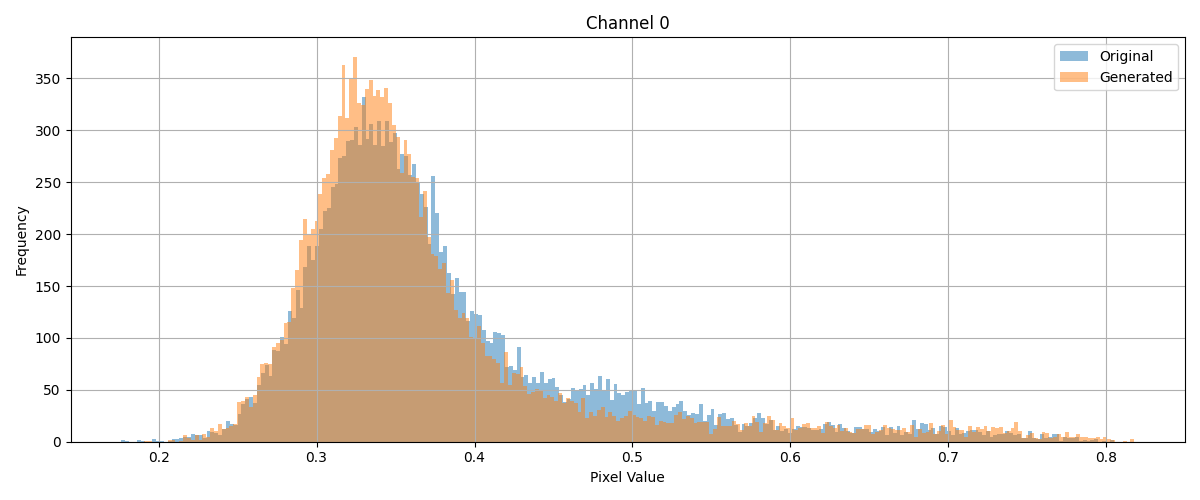
\includegraphics[width=0.9\textwidth]{images/distributions/cg_compare_distribution_5}
    \caption{Example of pixel value distribution comparison. Overlapping the histograms of Real (Target) and Generated data allows for the immediate detection of varying intensity scales or \enquote{mode collapse}, where the generator fails to capture the full dynamic range of the radar signal.}
    \label{fig:pixel_distribution}
\end{figure}

This diagnostic is critical for ensuring that the CycleGAN effectively aligns the \textit{marginal distributions} of the two domains.
A discrepancy in the histogram tails, for instance, often indicates that the model is failing to reproduce the decay characteristic of the Martian surface, or is truncating the noise floor.

\subsection{Range-Line Intensity Profiling}
A unique characteristic of radar sounding data is the physical attenuation of the signal with depth.
To verify that the generator learns this physical law—rather than simply performing style transfer on surface features—we introduced a \textbf{Range-Line Intensity Profile} evaluation (\texttt{src.utils.save\_rangeline\_comparison}).

This routine extracts a 1D vertical slice (A-scan) from the center of the generated radargram and compares it against the corresponding trace from the real target.
By overlaying these profiles, we can visually inspect:
\begin{itemize}
    \item \textbf{Surface Peak Matching:} Whether the generated surface return matches the amplitude and width of the real signal.
    \item \textbf{Attenuation Trend:} Whether the noise floor decays correctly with depth, mirroring the physical loss tangent of the crust. 
\end{itemize}
Discrepancies in the lower sections of this profile were instrumental in identifying the need for additional Z-score normalization in later stages of the pipeline.

\subsection{Evolutionary Trajectory Plotting}
To monitor the temporal stability of the learning process, the framework maintains a fixed \enquote{anchor} sample that is processed at every epoch.
The \texttt{plot\_evolution} module visualizes the trajectory of this specific sample throughout the training timesteps, arranging the snapshots in a chronological grid.
This visualization allows for the detection of \textit{cyclical forgetting}, where the model learns a feature (e.g., a specific speckle pattern) only to unlearn it in subsequent epochs due to the adversarial game's instability.


\section{Environment Isolation and Reproducibility}
\label{sec:reproducibility}

A defining characteristic of scientific software is reproducibility.
Deep learning experiments are notoriously sensitive to variations in the software stack, where differences in library versions or CUDA drivers can lead to non-deterministic numerical divergences.
To mitigate this, the entire training pipeline is containerized using \textbf{Docker}.

\subsection{Containerization Strategy}
The experimental environment is strictly defined via a \texttt{Dockerfile} that builds upon the official NVIDIA PyTorch image (\texttt{nvcr.io/nvidia/pytorch:24.06-py3})~\cite{nvidia_pytorch_docker}.
This base image provides a validated stack of low-level dependencies, including the CUDA Toolkit, cuDNN primitives, and NCCL communication libraries, optimized for the underlying GPU hardware.

By encapsulating the project dependencies (including specific versions of \texttt{PyTorch 2.4.0}, \texttt{Optuna}, and scientific libraries like \texttt{scikit-image}) within an immutable image, we guarantee that the code executes in an identical software context whether it is running on a local Windows development workstation or on a distributed Linux HPC cluster.
This approach elevates the project from a set of experimental scripts to deployable scientific software, ensuring that any researcher can replicate the exact experimental conditions by simply building the container.


\section{Automated Hyperparameter Optimization Framework}
\label{sec:hyperparameter_framework}

Identifying the optimal configuration for a GAN is a complex high-dimensional search problem.
To address this, an automated optimization infrastructure was integrated into the pipeline (\texttt{scripts/tune\_hyperparameters.py}), leveraging the \textbf{Optuna} framework~\cite{optuna_2019}.

\subsection{Optimization Strategy}
Instead of relying on inefficient Grid Search or Random Search methods, the framework utilizes a \textbf{Tree-structured Parzen Estimator (TPE)} sampler~\cite{optuna_2019}.
TPE is a Bayesian optimization algorithm that models the probability density function of the objective metric.
As the tuning process progresses, TPE learns which regions of the hyperparameter space are most likely to yield improvements, progressively concentrating the search on the most promising configurations.

\subsection{Search Space and Objective Function}
The optimization is defined over a specific Search Space (e.g., $LR_G \in [10^{-5}, 10^{-3}]$, where $LR_G$ denotes the generator learning rate, $\lambda_{cycle} \in [5, 20]$, where $\lambda_{cycle}$ weights the cycle-consistency loss).
The \textbf{Objective Function} defined for this study drives the TPE sampler to maximize the \textbf{Structural Similarity Index (SSIM)} on the validation set.
SSIM was selected as the target metric because, unlike pixel-wise Mean Squared Error, it correlates strongly with the preservation of structural geological features, guiding the search towards models that maintain stratigraphic integrity rather than just minimizing noise variance.


\section{Anomaly Detection Methodology}
\label{sec:anomaly_detection_methodology}
The primary application of the trained image-to-image translation models in this project is the unsupervised detection of subsurface anomalies in SHARAD radargrams.
To understand \textit{why} Image-to-Image (I2I) translation is exceptionally suited for this task, we must consider the physical limitations of our input data.

Upon training our model, we obtain a generator $G$ capable of converting a given simulated scenario (based purely on surface topography) into a highly realistic radargram.
Crucially, because the input simulations inherently lack any information about subsurface interfaces, the neural network learns to synthesize only the \enquote{normal} background distribution: surface clutter, speckle, and thermal noise.


Therefore, when we input a specific simulated radargram $x_{sim}$, the generator outputs a \enquote{blind} reconstruction $x_{gen} = G(x_{sim})$ that represents how the scene \textit{should} look if no subsurface geology were present.
By calculating the pixel-wise difference between this generated baseline $x_{gen}$ and the actual real-world observation $x_{real}$, genuine subsurface reflectors emerge as statistically significant residuals.
This approach effectively isolates the anomalies by subtracting the learned clutter.

The anomaly detection process is implemented in the \texttt{scripts/detect\_anomalies.py} script and follows a configurable pipeline, conceptually illustrated in Figure~\ref{fig:anomaly_detection_pipeline} and mirroring the final operational phase mapped in Block 4 of the general system architecture (Figure~\ref{fig:system_architecture2}):

\begin{figure}[htbp]
    \centering
    \begin{tikzpicture}[
        box/.style={rectangle, draw, minimum width=3cm, minimum height=1.2cm, align=center, thick, rounded corners=2pt},
        circle_op/.style={circle, draw, thick, minimum size=0.8cm, inner sep=0pt, align=center},
        textnode/.style={align=center},
        arrow/.style={-{Stealth}, thick}
    ]

    % --- RIGA 1: Generazione (Y = 0) ---
    \node[textnode] (sim)  at (0, 0) {Simulated \\ Radargram ($x$)};
    \node[box, fill=blue!10] (gen)  at (4, 0) {\textbf{Trained} \\ \textbf{Generator} ($G$)};
    \node[textnode] (fake) at (8, 0) {Generated \\ Background ($\hat{y}$)};

    % --- RIGA 2: Sottrazione (Y = -2) ---
    % Il nodo reale è perfettamente allineato sotto il generatore (X = 4)
    \node[textnode] (real) at (4, -2) {Real \\ Observation ($y$)};
    % Il nodo differenza è perfettamente allineato sotto il fake (X = 8)
    \node[circle_op, fill=yellow!20] (diff) at (8, -2) {$-$};

    % --- RIGA 3: Metriche (Y = -4) ---
    % L'output torna perfettamente in colonna con il generatore (X = 4)
    \node[textnode] (anomaly) at (4, -4) {Anomaly Map \\ (Residuals)};
    % La metrica è perfettamente in colonna con la differenza (X = 8)
    \node[box, fill=green!10] (metric) at (8, -4) {\textbf{Distance Metric} \\ (L1, L2, SSIM)};

    % ---- FRECCE ----
    \draw [arrow] (sim) -- (gen);
    \draw [arrow] (gen) -- (fake);
    
    \draw [arrow] (fake) -- (diff);
    \draw [arrow] (real) -- (diff);
    
    \draw [arrow] (diff) -- (metric);
    \draw [arrow] (metric) -- (anomaly);

    \end{tikzpicture}
    \caption{Flowchart of the proposed anomaly detection methodology. A simulated radargram ($x_{sim}$) is translated into a realistic background representation ($x_{gen}$) containing only noise and clutter. The difference between this generated baseline and the actual real-world observation ($x_{real}$) highlights un-modeled subsurface features, producing the final anomaly map.}
    \label{fig:anomaly_detection_pipeline}
\end{figure}

\subsection{Reconstruction and Difference Map Calculation}
Given an input simulated radargram $x_{sim}$, the trained generator produces a reconstructed baseline version $x_{gen}$ of its simulated counterpart.
The core of the anomaly detection process lies in quantifying the dissimilarity between this reconstruction and the ground truth real observation $x_{real}$.
To prevent edge artifacts and allow for the computation of perceptual metrics, the similarity evaluation is strictly performed on the full-resolution $128 \times 128$ images before any local aggregation takes place.
This is done by computing a \textbf{dense difference map $\mathcal{M}$}, which highlights the areas where the two images diverge.
This project supports several metrics for this purpose, each capturing different aspects of image similarity at the pixel-neighborhood level.

\begin{itemize}
    \item \textbf{L1 Distance (Mean Absolute Error):} The L1 distance measures the absolute difference between pixel values. It is a simple and effective way to capture the magnitude of errors. The L1 distance between the real observation $x_{real}$ and the generated background $x_{gen}$ is given by:
    $$ \mathcal{D}_{L1}(x_{real}, x_{gen}) = |x_{real} - x_{gen}| $$

    \item \textbf{L2 Distance (Mean Squared Error):} The L2 distance measures the squared difference between pixel values. Compared to L1, it penalizes larger errors more heavily.
    $$ \mathcal{D}_{L2}(x_{real}, x_{gen}) = (x_{real} - x_{gen})^2 $$

    \item \textbf{Structural Similarity Index (SSIM):} SSIM is a perceptual metric that considers luminance, contrast, and structure. The difference map can be computed as $1 - \text{SSIM}(x_{real}, x_{gen})$.

    \item \textbf{Learned Perceptual Image Patch Similarity (LPIPS):} LPIPS uses a deep network to compute a perceptually-aligned distance between the images~\cite{Zhang_2018_CVPR}.
\end{itemize}

\subsection{Anomaly Score Calculation Methods}
Once a difference map $\mathcal{M}$ is computed using one of the metrics described above, the raw values need to be aggregated into a coherent \enquote{Anomaly Score} that can be thresholded to make a binary decision.
The method used for this aggregation significantly impacts the spatial resolution and noise sensitivity of the detector.
We implemented and compared several distinct strategies.

\subsubsection{Pixel-Level Scoring}
This is the most granular approach, where the anomaly score $A_{i,j}$ at coordinates $(i,j)$ is simply the raw value of the anomaly map $\mathcal{M}_{i,j}$:
$$ A_{i,j} = \mathcal{M}_{i,j} $$
While this method preserves the maximum theoretical resolution, allowing for the detection of single-pixel anomalies, it is inherently unstable and sensitive to speckle noise.
Radar data is characterized by speckle noise, constructive and destructive interference patterns that vary stochastically.
A pixel-level difference can be high simply due to noise variance rather than a genuine geological discrepancy, leading to a "salt-and-pepper" distribution of False Positives.

\subsubsection{Patch-Based Aggregation}
To mitigate the noise sensitivity, the resulting difference map $\mathcal{M}$ is spatially aggregated using non-overlapping windows of size $k \times k$ (e.g., $16 \times 16$).
In practice, this is efficiently implemented as a 2D average pooling operation over the residual tensor.
The anomaly score for a patch $P$ is calculated as the mean intensity of the difference values within that region:
$$ A_P = \frac{1}{k^2} \sum_{(i,j) \in P} \mathcal{M}_{i,j} $$
This averaging acts as a low-pass filter, suppressing high-frequency noise.
However, it introduces a \enquote{blocking artifact} and reduces the effective spatial resolution.
If a small anomaly lies on the boundary between two patches, its energy is split, potentially causing both patches to fall below the detection threshold (False Negative).


\section{Synthetic Anomaly Injection Strategy}
\label{sec:synthetic_anomaly_injection}
Validating the performance of an anomaly detection system in a planetary exploration context presents a unique challenge: the absence of a comprehensive \enquote{Ground Truth}.
Unlike industrial inspection tasks where defects are known and labeled, the real Martian subsurface contains an unknown number of potential anomalies (indices of ice, voids, or distinctive stratigraphy), making it hard to calculate standard precision and recall metrics on real data alone.

To rigorously quantify the detector's discriminatory power, we developed a \textbf{Synthetic Anomaly Injection Strategy}.
This methodology relies on the controlled introduction of artificial, physically plausible perturbations into real observation samples ($x_{real}$).

The injection process is modeled as a transformation $T(x_{real})$ applied to real radargrams.
The procedure follows four physical constraints to simulate realistic \textbf{Dipping Layers} (inclined stratigraphic interfaces), which are common in regions like the North Polar Layered Deposits (NPLD):

\begin{enumerate}
    \item \textbf{Surface-Relative Positioning:} To mimic a subsurface layer, the anomaly's depth $d(x)$ is defined relative to the detected surface horizon $y_{surf}(x)$. For a column $x$, the anomaly position is:
    $$y_{anom}(x) = y_{surf}(x) + \delta_{start} + m \cdot (x - x_{start})$$
    where $\delta_{start}$ is a random initial depth offset and $m$ is the slope of the layer ($m \in [-0.5, 0.5]$).
    \item \textbf{Physical Attenuation Modeling:} Radar signals attenuate as they propagate through the crust. We model the intensity of the injected anomaly $I_{anom}$ not as a constant value, but as a fraction of the local surface power $I_{surf}$, reduced by an attenuation factor $\alpha$:
    $$I_{anom}(x) = I_{surf}(x) - \alpha$$
    where $\alpha \sim U(0.2, 0.6)$ ensures the anomaly is visible but not blatantly artificial, challenging the detector to distinguish it from background noise.
    \item \textbf{Stochastic Texture (Speckle):} A solid line would be trivial to detect and physically unrealistic. We inject a granular texture by adding Gaussian noise $\eta \sim \mathcal{N}(0, 0.1)$ to the layer intensity, simulating the constructive and destructive interference typical of coherent radar systems.
    \item \textbf{Constructive Interference Merging:} The anomaly is merged with the original observation $x_{real}$ using a maximum-power operator, simulating the dominance of the strongest reflector in a resolution cell:
    $$ x_{injected}(i, j) = \max(x_{real}(i, j), I_{anom}(i, j) \cdot M_{GT}(i, j)) $$
\end{enumerate}

Simultaneously with the injection, we generate a pixel-perfect binary mask $M_{GT}$, where $M_{GT}(i,j)=1$ if the pixel $(i,j)$ was modified, and 0 otherwise.
These \enquote{corrupted} real observations ($x_{injected}$) are then passed through the standard detection pipeline: they are compared against the generator's reconstruction of the corresponding pristine simulation ($x_{gen} = G(x_{sim})$), and the residual map $\mathcal{M}$ is computed.
By comparing the calculated anomaly score map $\mathcal{M}$ against the binary $M_{GT}$, we can perform a quantitative Receiver Operating Characteristic (ROC) analysis.

\subsection{Automated Evaluation Protocol}
\label{subsec:auto_eval_protocol}
To rigorously quantify the detector's capabilities without relying on manual inspection, we developed an automated evaluation protocol (implemented in \texttt{scripts/evaluate\_anomalies.py}).
This script executes the following pipeline on a held-out test set (which, as will be detailed in Section~\ref{subsec:roi_selection}, complements the manually curated real observations with this synthetically corrupted dataset):

\begin{enumerate}
    \item \textbf{Dynamic Injection:} For each test sample, a synthetic anomaly (e.g., a dipping layer) is injected into the real observation $x_{real}$ with randomized parameters (depth, slope, attenuation), producing an altered radargram denoted as $x_{injected}$.
    \item \textbf{Reconstruction \& Residuals:} The generator reconstructs the \enquote{background-only} estimate $x_{gen} = G(x_{sim})$ \textbf{from the simulated} radargram $x_{sim}$, and the absolute difference anomaly map $\mathcal{M} = | x_{injected} - x_{gen} |$ is computed.
    \item \textbf{Metric Aggregation:} The pixel-level anomaly scores from $\mathcal{M}$ are compared against the ground-truth binary mask $M_{GT}$ of the injected anomaly.
\end{enumerate}

We utilize standard information retrieval metrics, based on Receiver Operating Characteristic (ROC) and Precision-Recall (PR) analyses, to benchmark the detector's sensitivity:
\begin{itemize}
    \item \textbf{Area Under the ROC Curve (AUC):} A threshold-independent measure of the detector's probability to rank a randomly chosen anomalous pixel higher than a background pixel.
    \item \textbf{Average Precision (AP):} Computed as the area under the PR curve. This metric is particularly sensitive to the false positive rate, making it the preferred metric for our highly imbalanced dataset (where anomalous pixels represent $<1\%$ of the total area).
\end{itemize}

The framework reports both the mean AUC/AP across the dataset and generates global ROC/PR curves to characterize the overall system performance.


\section{Conclusion}
The methodology detailed in this chapter, from the physics-aware data pre-processing to the containerized, modular deep learning implementation, establish a robust foundation for the experiments.
By automating data ingestion, ensuring memory safety through chunking, and rigorously isolating the execution environment via Docker, we have minimized computational overhead and procedural errors and maximized the scientific validity of the results.
Furthermore, the integration of the Optuna optimization framework enables a systematic exploration of the model's parameters space, ensuring that the configurations used in the subsequent analysis are data-driven rather than arbitrary.
The following chapter will present the quantitative and qualitative outcomes of our experiments, demonstrating the effectiveness of the proposed CycleGAN approach in translating synthetic images into realistic observations for the ultimate goal of unsupervised subsurface anomaly detection.


